%==============================================================================
% TRB 2027 投稿 —— 英文正式版
%
% ▶ 本文件 = 英文投稿工作稿。中文工作稿 `729-paper-中文版.tex` 是内容真相源，
%   本文件只做「选进 20 页的那部分」的英文表达，**不是逐句直译**。
% ▶ 编译：`pdflatex 801-paper-英文版.tex`（跑两次更新交叉引用与 pagewise 行号）。
%   纯英文 ⟹ 不需要 xelatex / xeCJK。
%
% ▶ 🔴 TRB 官方硬要求（逐条见 `04 §九`）：
%   · 总共 20 页，标题页 + 摘要页 + 正文 + 致谢 + 参考文献 + 全部图表都算在内。
%   · Times New Roman ≥10 pt · 单栏 · 单倍行距 · 8.5×11 in · 四边 1 in 页边距。
%   · 每页行号从 1 重新计数 · 页码每页底部居中 · 图表嵌在讨论它的段落附近。
%   · 引用 (Author, Year) · **不允许附录 / 补充材料**。
%   · 摘要 ≤300 词、独占第 2 页、五个加粗小标题按序、不含图表公式与未定义缩写。
%
% ▶ 字号：官方 Word 样例 `_模板_官方Word原版_TAD_AMSamplePaper.docx` 实测
%   正文 Normal = **11 pt**（styles.xml docDefaults w:sz=22 半磅）、Heading1 = 12 pt 加粗。
%   中文工作稿用的是 12 pt（比官方样例大一号）。本文按官方样例取 11 pt。
%
% ▶ 🔴 写作红线（CLAUDE.md §0 · 一个字不能松）：
%   能严证 = 远场单步无碰 + 每让路步方向合规 + 紧急迫近不可避的 sound 证书。
%   绝不写 provably collision-free / 裸的 provably compliant / zero collisions。
%   一律写 provable **directional** compliance，并写明作用域。
%
% ▶ 英文行文（user 2026-08-01 明令）：严格学术英语，**只用简单句**，避免长难句，
%   以「普通读者读得懂」为准。
%==============================================================================
% 🔴 2026-08-01 later-6：由 11 pt 改 10 pt。
%    §1/§2/§6/§7 补齐之后 11 pt 排出来 **23 页**，硬上限是 20 页。
%    10 pt 实测 **20 页**（TRB 硬要求是 ≥10 pt，10 pt 合规，是 `04 §九` 早就写好的退路）。
%    仍不够：图 1 总览、图 6 轨迹、致谢/作者贡献/利益冲突/资助 还没进来，约再占 2 页 ⟹ 还要砍。
%    要退回 11 pt 就把下面这行的 10pt 改回 11pt，一行的事。
\documentclass[10pt,letterpaper]{article}

%--- 数学 ---------------------------------------------------------------------
\usepackage{amsmath}
\usepackage{amssymb}
\usepackage{bm}
\usepackage{amsthm}
\newtheorem{prop}{Proposition}

%--- 字体：Times 风格（正文与公式）---------------------------------------------
\usepackage[T1]{fontenc}
\usepackage[utf8]{inputenc}
\usepackage{mathptmx}

%--- 页面：US Letter，四周 1 英寸页边距 ----------------------------------------
\usepackage[letterpaper,margin=1in,headheight=15pt,headsep=0.25in,footskip=0.3in]{geometry}

%--- 页眉（斜体 running head）+ 页脚（居中页码·官方硬要求）---------------------
\usepackage{fancyhdr}
\pagestyle{fancy}
\fancyhf{}
\fancyhead[L]{\itshape Tang, Xue, Yang, and Li}
\fancyfoot[C]{\thepage}
\renewcommand{\headrulewidth}{0pt}
\renewcommand{\footrulewidth}{0pt}

%--- 正文：两端对齐、单倍行距、首行缩进、段间不额外加空 -------------------------
%  🔴 2026-08-01 订正（user 指出 + 实测官方 Word 样例坐实）：
%     样例里唯一写了字的正文（那份结构化摘要四段）**全部是 jc=both 两端对齐**；
%     Lorem ipsum 那些占位段没写 jc（继承为左对齐），但占位文的排版不作数。
%     先前照 LaTeX 模板注释用了 \RaggedRight，是照抄模板作者的偏好、不是官方规定。⟹ 改回两端对齐。
%  首行缩进：官方样例 w:ind firstLine=720 twip = 0.5 in（24 段实测）。
\usepackage{ragged2e}
\setlength{\parindent}{0.5in}
\setlength{\parskip}{0pt}

%--- 标题层级：**复原官方 TAD 模板**（中文工作稿为可读性加了编号与放大，投稿版不留）--
\usepackage{titlesec}
%  🔴 编号开关（user 2026-08-01：「你先听我的这样做，我这样能看得清楚你的文章结构」）
%     \SECNUM = 1 ⟹ 一二三级标题带编号（当前，写作期用，方便对结构）
%     \SECNUM = 0 ⟹ 官方 TAD 样例原样：标题**不编号**
%     🔴 投稿前必须改回 0（官方样例实测：全篇标题无编号）。改一个字符即可，别动下面的格式。
\newcommand{\SECNUM}{1}
%
%  三级标题的**格式**照官方 Word 样例实测值，编号与否不影响格式：
%    一级 \section       = 12 pt 加粗 + 全大写（Heading1）
%    二级 \subsection    = 11 pt 加粗（正文字号，Heading2）
%    三级 \subsubsection = 11 pt 斜体（正文字号，Heading3）
%    四级                 = 段首加粗引导词，与正文同一段（run-in，不占一行）
\ifnum\SECNUM=1
  \setcounter{secnumdepth}{3}
  \titleformat{\section}{\normalfont\fontsize{12}{14}\selectfont\bfseries}{\thesection\quad}{0pt}{\MakeUppercase}
  \titleformat{\subsection}{\normalfont\bfseries}{\thesubsection\quad}{0pt}{}
  \titleformat{\subsubsection}{\normalfont\itshape}{\thesubsubsection\quad}{0pt}{}
\else
  \setcounter{secnumdepth}{0}
  \titleformat{\section}{\normalfont\fontsize{12}{14}\selectfont\bfseries}{}{0pt}{\MakeUppercase}
  \titleformat{\subsection}{\normalfont\bfseries}{}{0pt}{}
  \titleformat{\subsubsection}{\normalfont\itshape}{}{0pt}{}
\fi
\titlespacing*{\section}{0pt}{12pt}{4pt}
\titlespacing*{\subsection}{0pt}{12pt}{4pt}
\titlespacing*{\subsubsection}{0pt}{12pt}{4pt}

%--- 图表 ---------------------------------------------------------------------
\usepackage{graphicx}
\usepackage{booktabs}
\usepackage{array}
\usepackage{multirow}
\usepackage{caption}
\usepackage{algorithm}
\usepackage[noend]{algpseudocode}
\renewcommand{\topfraction}{0.9}
\renewcommand{\bottomfraction}{0.7}
\renewcommand{\textfraction}{0.08}
\renewcommand{\floatpagefraction}{0.8}
\setcounter{topnumber}{3}
\setcounter{totalnumber}{4}
\captionsetup[algorithm]{labelsep=space,labelfont=bf,font=small}
\captionsetup{labelsep=space,font=bf,justification=raggedright,singlelinecheck=false}
\captionsetup[table]{name=TABLE}
% 图/表的【名字】随官方样例保持粗体正文号；后面的【说明】降一号（10 pt）且不加粗。
% 🔴 TRB 硬要求是 Times New Roman ≥10 pt ⟹ \small（11pt 基准下 = 10 pt）是**下限**，
%    再小就不合规。所以说明只能降到 10 pt，不能更小。
\newcommand{\capnote}[1]{{\normalfont\small #1}}
\captionsetup[figure]{name=Figure}
\usepackage{placeins}   % \FloatBarrier：把待排的图表在此之前全部排掉，别溢进参考文献

%--- 超链接：hidelinks = 可跳转但引用文字保持黑色（user 要求）-------------------
\usepackage[hidelinks]{hyperref}

%--- 行号：TRB 硬要求，pagewise = 每页从 1 重新计数 ----------------------------
\usepackage[left,pagewise]{lineno}
\renewcommand{\linenumberfont}{\normalfont\small}

%--- 摘要小标题 ---------------------------------------------------------------
\newcommand{\abshead}[1]{\textbf{#1}\ }

%--- 参考文献：Chicago 作者-年份、按第一作者姓氏字母序、悬挂缩进、不编号 ---------
\newcommand{\refitem}[1]{\par\begingroup\emergencystretch=3em\sloppy\noindent\hangindent=0.5in\hangafter=1 #1\par\endgroup}
\newcommand{\cit}[1]{(#1)}
\newcommand{\citp}[2]{(#1 #2)}
%--- 可跳转引用（user 要求：文献可点击，引用文字保持黑色；hyperref 已是 hidelinks）------
%  \citl{键}{显示文字}  单条 · \citm{\cl{k1}{A 1999}; \cl{k2}{B 2020}} 多条 · 锚点在 _refs.tex
\newcommand{\citl}[2]{(\hyperlink{ref:#1}{#2})}
\newcommand{\citm}[1]{(#1)}
\newcommand{\cl}[2]{\hyperlink{ref:#1}{#2}}

%--- 占位宏 -------------------------------------------------------------------
\newcommand{\figplaceholder}[1]{\fbox{\parbox[c][6cm][c]{\dimexpr\linewidth-2\fboxsep-2\fboxrule}{\centering\textbf{[#1 placeholder]}}}}
\newcommand{\TBD}{[TBD]}
\newcommand{\prov}[1]{#1}

%==============================================================================
\begin{document}
\linenumbers

%------------------------------------------------------------------------------
% 第 1 页：标题页（官方要求：标题 + 全部作者姓名/职称/单位/邮箱 + 总页数）
%------------------------------------------------------------------------------
\begin{flushleft}
{\bfseries Half-Plane Shielding: Provable Directional COLREGs Compliance for Continuous-Action Safe Reinforcement Learning}\par
\vspace{12pt}

{\bfseries Weiyu Tang}\par
Graduate Research Assistant\par
Shanghai Key Laboratory for Digital Maintenance of Buildings and Infrastructure,\par
School of Naval Architecture, Ocean and Civil Engineering\par
Shanghai Jiao Tong University, Shanghai, 200240, China\par
Email: weiyutang@sjtu.edu.cn\par
\vspace{12pt}

{\bfseries Jie Xue, Ph.D.\textsuperscript{*}}\par
Assistant Research Professor\par
State Key Laboratory of Ocean Engineering\par
School of Naval Architecture, Ocean and Civil Engineering\par
Shanghai Jiao Tong University, Shanghai, 200240, China\par
Email: j.xue@sjtu.edu.cn\par
\vspace{12pt}

{\bfseries Peijie Yang}\par
Shanghai Key Laboratory for Digital Maintenance of Buildings and Infrastructure,\par
School of Naval Architecture, Ocean and Civil Engineering\par
Shanghai Jiao Tong University, Shanghai, 200240, China\par
Email: yangpeijie21@sjtu.edu.cn\par
\vspace{12pt}

{\bfseries Qianbing Li}\par
Shanghai Key Laboratory for Digital Maintenance of Buildings and Infrastructure,\par
School of Naval Architecture, Ocean and Civil Engineering\par
Shanghai Jiao Tong University, Shanghai, 200240, China\par
Email: qianbing\_li@sjtu.edu.cn\par
\vspace{12pt}

Word Count: \TBD\ words + \TBD\ table(s) $\times$ 250 = \TBD\ words\par
Total Number of Pages: \TBD\par
\vspace{24pt}

Submitted [Submission Date]\par
\textsuperscript{*}Corresponding Author\par
\end{flushleft}

\newpage

%------------------------------------------------------------------------------
% 第 2 页：结构化摘要（≤300 词 · 独占一页 · 五个加粗小标题按序 · 不含图表公式）
%------------------------------------------------------------------------------
\section*{Abstract}
%  🔴 2026-08-01 实测官方 Word 样例（`_模板_官方Word原版_TAD_AMSamplePaper.docx` 的 document.xml）：
%     摘要那五段 **w:ind 一律 none（零缩进）+ w:jc=both（两端对齐）**；
%     正文段才有 w:firstLine="720"（=0.5 in）。
%     ⟹ 摘要页把首行缩进关掉，出这一页再恢复。小标题用**冒号**，也是照样例。
\begingroup
\setlength{\parindent}{0pt}

\abshead{Objectives:}Autonomous surface vessels must obey the International Regulations for Preventing Collisions at Sea (COLREGs). The give-way rules are directional. A track that avoids a collision but passes on the wrong side still violates them. This paper builds a per-step guarantee of directional compliance for continuous control.

\abshead{Methods:}The give-way clause is written as a half-plane constraint on the plane of control commands. It is intersected with the actuator limits and a one-step collision-free condition, which gives a convex safe control set. A small quadratic program projects the command of the policy onto the nearest point of that set. The projection sits inside the environment transition, so the policy learns under its own corrected commands. The data are 2,000 simulated two-vessel encounters, split into 1,400 training and 600 test cases. Nine configurations form a single-variable ladder, each trained with eight seeds.

\abshead{Findings:}On every give-way step where the projection is feasible, directional compliance holds by construction, independently of the training outcome and the seed. Fallback steps are not covered. On the 600 test scenarios the median violation count is 0.53 per episode, against 1.16 for a discrete shielded baseline, at a median collision rate of 0.00\%. The ablation gains are significant under a paired signed-rank test. The arrival rate is not claimed as a benefit.

\abshead{Novelty:}To the best of the authors' knowledge, this is the first projection-based safety mechanism that enforces directional COLREGs compliance on continuous control. The paper also states what is proved and what is not.

\abshead{Practical Applications:}The compliance check is independent of training. It can sit above an existing controller as a compliance layer for functional verification and liability assessment. The online cost is one small quadratic program per step, which runs in real time without special hardware.

\vspace{12pt}

\endgroup

\noindent\textbf{Keywords:} COLREGs compliance, safe reinforcement learning, projection-based safety shield, continuous action space, quadratic programming, unmanned surface vehicle


\newpage

%==============================================================================
% 正文 —— 本轮**只做固定开销**（标题页 / 摘要页 / 参考文献），用来量真实剩余额度。
%
% 🔴 2026-08-01 实测（本文件这套版式，pdflatex 真编译，不是估算）：
%   固定开销：11 pt = **5 页**（标题 1 + 摘要 1 + 参考文献 3）· 10 pt = **4 页**（参考文献 2）
%   正文文字容量：10 pt ≈ 870 词/页 · 11 pt ≈ 644 词/页 · 12 pt ≈ 561 词/页
%   中文正文 15,717 汉字（含图表标题与图注）· 实测折算率 1.71 汉字/词（本文摘要中英对照：505 字 = 296 词）
%   ⟹ 中文正文全译 ≈ 9,200 英文词 ⟹ 11 pt 下要 14.3 页，10 pt 下要 10.6 页。
%
% ⟹ 20 页总额下的正文文字额度（图表按 04 §九 的 7 页估）：
%   11 pt：20 − 5 − 7 = **8 页 ≈ 5,150 词** ⟹ 只装得下现有正文的约 **56%**
%   10 pt：20 − 4 − 7 = **9 页 ≈ 7,830 词** ⟹ 装得下约 **85%**
%   👉 砍多少取决于字号这个开关，**先定字号再定砍谁**。图表那 7 页要单独实测，别一直用估值。
%
% 正文按砍定的清单逐节补进来；节序沿用中文稿：
%   Introduction / Related Work / Problem Formulation / Methodology /
%   Experiments / Discussion / Conclusions / Acknowledgements /
%   Author Contributions / Conflict of Interest / Funding
%==============================================================================


%==============================================================================
% §1 引言 —— 对应中文稿 249–266 行
%==============================================================================
\section{Introduction}
\label{sec:intro}

Two vessels meet at sea. Each turns to starboard, and they pass clear of one another. What
makes this work is not the judgment of either bridge team. It is a set of rules that both
sides follow, and that both sides know the other will follow. When no one is on board, that
predictability becomes a technical requirement. A maritime inquiry does not only ask whether
contact occurred. It also asks whether the vessel acted as the rules require. An encounter
that ends without contact but passes on the wrong side is still recorded as a breach.

Collision avoidance for autonomous surface vessels must therefore satisfy the International
Regulations for Preventing Collisions at Sea \citl{imo1972}{IMO 1972}. One property of that
rule set decides the shape of the problem. The give-way clauses are
\textbf{directional}. In a head-on encounter both vessels turn to starboard. In a crossing
encounter the give-way vessel turns to starboard and the stand-on vessel holds course and
speed. In an overtaking encounter the overtaking vessel keeps clear. A control command can
therefore avoid contact and still break the rules, because it turned the wrong way.
Compliance cannot be verified from the outcome. It is a condition on which half-plane of the
control plane each command falls in, and that is not the usual shape of a constraint in safe
reinforcement learning.

Existing work follows two routes, and each gives up one property. The first discretizes
the action space and masks the non-compliant commands \citl{krasowski2024}{Krasowski and
Althoff 2024}. Compliance then holds by construction, and it does not depend on the
training outcome or on the seed. The price is continuous control. Quantization fixes the control resolution at the grid spacing. A give-way turn that must
be readily apparent has a smallest admissible turn rate, and no finite grid lands on it,
so every compliant turn overshoots. The second route keeps continuous control and writes the
rules into the reward as a penalty \citm{\cl{meyer2020}{Meyer et al. 2020};
\cl{heiberg2022}{Heiberg et al. 2022}; \cl{mller2026}{M\"uller et al. 2026}}. Control
resolution is preserved and the guarantee is lost, because a reward shapes expected
behavior and cannot exclude any single violating command. Section~\ref{sec:related} sets
out both routes in detail.

The intersection of continuous action spaces, provable directional compliance and COLREGs
has therefore been empty. This paper fills it with a projection-based safety shield. A rule
state machine returns the half-plane of compliant directions. That half-plane is intersected
with the action box and with a one-step collision-free condition, which gives a convex safe
control set. A quadratic program projects the continuous command of the policy onto the
nearest point of that set. The step that makes this possible is a change of premise. Action
masking needs the safe set to be enumerable. Projection needs it only to be convex. The
shield sits inside the environment transition, so the policy learns under its own corrected
commands.

The second concern of this paper is the scope of what is proved. The word provable covers
different scopes in the safe reinforcement learning literature, and those scopes do not
always match what a reader assumes. Each guarantee below is therefore stated with its
assumptions, and the cases that are not covered are stated as well.

\noindent\textbf{Contributions.}
\begin{enumerate}\itemsep2pt
 \item A projection-based COLREGs shield for continuous action spaces
 (Section~\ref{sec:proj}).  The compliant direction enters the quadratic program as a hard constraint. Directional
 compliance therefore holds by construction on every give-way step where the projection
 is feasible. It does not depend on the training outcome or on the seed.
 \item A graded safety statement (Section~\ref{sec:collfree}). One-step collision freedom in
 the far field is a strict result. Directional compliance on every feasible give-way step
 holds by construction. Imminent unavoidable collision is flagged by a sufficient
 condition that never raises a false alarm. Each statement carries its assumptions, and the
 uncovered cases are named.
 \item An experimental design that separates the mechanisms (Section~\ref{sec:setup}). Nine
 configurations form one connected single-variable ladder. Three steps of that ladder carry
 a companion variable that cannot be separated, and those are listed with the ladder.
\end{enumerate}

%==============================================================================
% §2 相关工作 —— 对应中文稿 268–320 行
%==============================================================================
\section{Related Work}
\label{sec:related}

\subsection{Maritime Collision Avoidance and COLREGs Compliance}

Work on rule compliance began with model-driven methods. The velocity obstacle uses the
relative velocity cone to select an avoiding velocity, and it was given COLREGs
semantics \citl{kuwata2014}{Kuwata et al. 2014} and later extended to more general
encounters \citl{huang2019}{Huang et al. 2019}. Model predictive control scores candidate
maneuvers over a finite horizon on both risk and compliance
\citl{johansen2016}{Johansen et al. 2016}. Its branching-course variant has been tested at
sea \citl{eriksen2019}{Eriksen et al. 2019} and at full scale
\citl{kufoalor2020}{Kufoalor et al. 2020}. An earlier protocol-based method wrote the rules
as an agreement negotiated between vessels
\citl{benjamin2006}{Benjamin et al. 2006}. Recent work on this route uses control barrier
functions and convex optimization \citm{\cl{lee2025}{Lee et al. 2025};
\cl{patil2026}{Patil et al. 2026}}, mostly on standard maneuvering models
\citl{fossen2011}{Fossen 2011}. Their guarantees come from explicit constraints. The control
law is designed by hand and contains no learned policy.

Deep reinforcement learning moved the policy into the data \citl{sarhadi2022}{Sarhadi et
al. 2022}. Most of that work discretizes the command, into a finite set of rudder angles
for confined water \citl{shen2019}{Shen et al. 2019}, or into compliant avoidance timing
and paths
\citm{\cl{zhao2019}{Zhao and Roh 2019}; \cl{chun2021}{Chun et al. 2021}}. Discretization
helps optimization and fixes control resolution at the grid spacing. A second group keeps
continuous control and writes COLREGs as a soft penalty that decays with bearing and range
\citl{meyer2020}{Meyer et al. 2020}, or as a tunable risk gate
\citl{heiberg2022}{Heiberg et al. 2022}. Compact reinforcement learning for obstacle
avoidance has also been shown on underactuated craft
\citl{cheng2018}{Cheng and Zhang 2018}. This group is usually built on proximal policy
optimization \citl{schulman2017}{Schulman et al. 2017}, and a bounded Beta distribution
\citl{chou2017}{Chou et al. 2017} can parameterize the continuous command so that samples
are not clipped at the boundary of the action box. Control resolution is preserved. Rule
compliance is induced by the reward, so no single violating command is excluded.

\subsection{Safe Reinforcement Learning and Provable Compliance}

Safe reinforcement learning \citl{garca2015}{Garc\'ia and Fern\'andez 2015} attaches
hard guarantees to a learned policy. Writing safety as a constrained Markov decision
process and solving it with a Lagrangian method guarantees constraint satisfaction in
expectation, which again excludes no single command. Action
masking removes unsafe commands from a discrete action space according to a temporal logic
specification \citl{alshiekh2018}{Alshiekh et al. 2018}. A realizable form of it has been
extended to continuous action spaces for general tasks, without maritime rules
\citl{kim2024}{Kim et al. 2024}. In continuous control, quadratic programs built on control
barrier functions \citl{ames2019}{Ames et al. 2019} and predictive safety shields
\citl{wabersich2021}{Wabersich and Zeilinger 2021} give per-step hard guarantees. The latter
has been attached to maritime reinforcement learning, where it constrains collision only and
carries no directional clause \citl{vaaler2024}{Vaaler et al. 2024}. The closest mechanism is a safety shield that linearizes the constraint at the current
state. It then projects the command of the policy onto the resulting half-space in
closed form \citl{dalal2018}{Dalal et al. 2018}. The projection used here has the same form. What is added is the encoding of the directional give-way clause as a half-plane in the
control plane. The enforced object is then rule compliance rather than a state bound.

Table~\ref{tab:related} places this work on four dimensions and shows where the gap is. A hard guarantee of rule compliance in a maritime setting had been demonstrated only on
a discrete action space \citl{krasowski2024}{Krasowski and Althoff 2024}. That work
provides the scenario library and the state machine thresholds used here. Action
projection under continuous control is listed there as future work
\citl{kochdumper2023}{Kochdumper et al. 2023}. Later work on that direction moved to
continuous control but approximated compliance with a soft reward, without a hard guarantee
\citl{mller2026}{M\"uller et al. 2026}. The present work gives a constructive guarantee of
directional compliance under continuous control. The reachable set is represented by a
convex over-approximation and the correction by a quadratic program
\citl{markgraf2026}{Markgraf et al. 2026}, rather than by a higher-order set representation, which keeps
the per-step cost small.

A directional constraint tightens the feasible set in close quarters and can cost
terminal efficiency. Potential-based shaping recovers it without changing the set of
optimal policies \citl{ng1999}{Ng et al. 1999}. A distance potential alone leaves a stalling mode near the goal \citl{trott2019}{Trott
et al. 2019}, which a single continuous potential does not remove
\citl{mller2025}{M\"uller and Kudenko 2025}. A linear kernel with arrival as a terminal
condition is used instead \citl{de2024}{De Lellis et al. 2024}. The effect of a shield on
performance has been studied separately. Including the filter during training and penalizing
the correction improves sample efficiency
\citl{pizarro2025}{Pizarro Bejarano et al. 2025}, a sufficiently permissive filter does not
cost asymptotic optimality \citl{oh2025}{Oh et al. 2025}, and a safety term that opposes the
goal term causes stalling short of the goal \citl{grover2023}{Grover et al. 2023}.

%------------------------------------------------------------------------------
\begin{table}[htbp]
 \caption{Position of related work. \capnote{A per-step hard guarantee means the class of
 commands the method can exclude at \emph{every} decision step, not constraint satisfaction
 in expectation.}}
 \label{tab:related}
 \centering\small
 \setlength{\tabcolsep}{3pt}
 \begin{tabular*}{\linewidth}{@{\extracolsep{\fill}}lllcc@{}}
  \toprule
  Representative work & Action space & Compliance is imposed by & Per-step guarantee & Learned \\
  \midrule
  \multicolumn{5}{@{}l}{\textit{Model-driven, no learning}}\\
  \citl{kuwata2014}{Kuwata et al. 2014} & Continuous & Velocity obstacle geometry & Geometric & - \\
  \citl{johansen2016}{Johansen et al. 2016} & Branches & Cost ranking & - & - \\
  \citm{\cl{lee2025}{Lee et al. 2025}; \cl{patil2026}{Patil et al. 2026}} & Continuous & Barrier function & State bound & - \\
  \midrule
  \multicolumn{5}{@{}l}{\textit{Learning, compliance from a soft reward}}\\
  \citl{meyer2020}{Meyer et al. 2020} & Continuous & Soft reward & - & $\checkmark$ \\
  \citl{heiberg2022}{Heiberg et al. 2022} & Continuous & Soft reward, risk gate & - & $\checkmark$ \\
  \citl{mller2026}{M\"uller et al. 2026} & Continuous & Soft reward, falsification & - & $\checkmark$ \\
  \midrule
  \multicolumn{5}{@{}l}{\textit{Learning, compliance from a hard constraint}}\\
  \citl{alshiekh2018}{Alshiekh et al. 2018} & Discrete & Action masking & State bound & $\checkmark$ \\
  \citl{dalal2018}{Dalal et al. 2018} & Continuous & Linearize, then project & State bound & $\checkmark$ \\
  \citl{vaaler2024}{Vaaler et al. 2024} & Continuous & Predictive safety shield & Collision only & $\checkmark$ \\
  \citl{krasowski2024}{Krasowski and Althoff 2024} & Discrete ($49$) & Action masking & \textbf{Direction} & $\checkmark$ \\
  \midrule
  \textbf{Ours} & \textbf{Continuous} & \textbf{Projection (QP)} & \textbf{Direction} & $\checkmark$ \\
  \bottomrule
 \end{tabular*}
\end{table}
%------------------------------------------------------------------------------

%==============================================================================
% §3 问题表述 —— 对应中文稿 323–422 行
%   🔴 砍掉了中文稿的**符号表**（tab:notation，30 余行）。20 页无附录，一张符号表就吃掉近一页；
%      改为符号在首次出现处随文交代。这是内容取舍，已记在 `英文写作规范.md`。
%==============================================================================
\section{Problem Formulation}
\label{sec:problem-setup}

\subsection{Vessel Kinematics}
\label{sec:model}

The controlled vessel is modeled as a point mass with a yaw constraint. Its state is
$s=[p_x,p_y,\theta,v]^{\!\top}\in\mathbb{R}^4$, which collects position, heading, and speed.
Its controls are the longitudinal acceleration $a$ and the turn rate $\omega$,
\begin{equation}
 \dot s=\bigl[\,v\cos\theta,\ \ v\sin\theta,\ \ \omega,\ \ a\,\bigr]^{\!\top},
 \qquad u=[a,\omega]^{\!\top}.
 \label{eq:dyn}
\end{equation}
The controls obey $|a|\le a_{\max}$ and $|\omega|\le\omega_{\max}$, and the speed obeys
$0\le v\le v_{\max}$. A command is held constant over one decision period $\Delta t$.
Headings and bearings are wrapped to $(-\pi,\pi]$. A relative bearing is positive to
starboard. The turn rate follows the usual mathematical convention and is positive
counter-clockwise, so a turn to starboard has $\omega<0$.

The speed bound is applied after integration, so the speed can briefly exceed $v_{\max}$
within a step. Every one-step displacement bound in this paper therefore uses
$v_{\max}\Delta t+\tfrac12 a_{\max}\Delta t^2$, and the speed at the end of a step is at
most $v_{\mathrm{bnd}}=v_{\max}+a_{\max}\Delta t$.

Two reasons fix this level of detail. The give-way rules govern changes of course and of
speed, and Equation~\eqref{eq:dyn} takes both as control commands. The rules can therefore be
written as constraints on $u$ with nothing in between, and that is what lets the whole
safety mechanism live in the action space. A finer hydrodynamic model would add
coefficients that differ by vessel and are hard to identify, and the rule constraints would
then be entangled with vessel parameters. Wind, current, and waves are not modeled.

\noindent\textbf{Vessel and occupancy.}\ The subject is a large container vessel of length
$175$~m and beam $25.4$~m. Its limits are $a_{\max}=0.24~\mathrm{m/s^2}$,
$\omega_{\max}=0.03$~rad/s, and $v_{\max}=9.5$~m/s. The decision period is $10$~s, and an
episode lasts at most $170$ steps, which is $1{,}700$~s. The circumscribed radius of the
hull is $88.4$~m and the inscribed radius is $12.7$~m.

The turn rate limit is about $1.7^\circ$ per second. A readily apparent turn of $20^\circ$
therefore needs more than ten seconds, which is longer than one decision period. The vessel
maneuvers more slowly than it decides. A safety constraint must look ahead for that reason
alone.

The hull is a rectangle, and two circles approximate it for two purposes. The circumscribed
circle over-approximates it and supports conditions of the form ``contact is impossible''.
The inscribed circle under-approximates it and supports conditions of the form ``contact is
certain''. One circle in each direction is
what keeps both kinds of conclusion one-sided. The target vessel is represented by a
rectangle as well, and it is extrapolated at constant velocity whenever a prediction is
needed.

\subsection{Observation and Action Spaces}
\label{sec:obsact}

The observation is a real vector of $27$ entries in four groups. Four give the state of
the own vessel, six the relation to the goal, twelve the traffic situation, and five are
termination flags. The traffic group uses four bearing sectors. Each contributes the nearest target vessel
in it, with its distance, its relative bearing, and the change of that distance over one
step. The observation layer outputs raw
physical quantities and the training wrapper normalizes them. Organizing traffic by
sector keeps the dimension independent of the number of target vessels. That solves the dimension only. The shield
deployed here is implemented for a single target vessel, and it raises an error rather than
running in a degraded mode when more are present.

\noindent\textbf{Two action boxes.}\ The action is the two-dimensional command
$u=(a,\omega)$, and two boxes have to be distinguished. The policy acts in the narrower
operating box, whose half-widths are $0.048~\mathrm{m/s^2}$ and $0.018$~rad/s. These are
exactly the span of the $7\times7$ grid used by the discrete configurations, so the two
action spaces carry the same control authority and differ only in resolution. The shield
and the emergency controller act in the wider box of the actuator limits,
$U_{\mathrm{box}}=\{|a|\le a_{\max}\}\cap\{|\omega|\le\omega_{\max}\}$.

The widening is necessary. A shield confined to the narrow box would declare a step
infeasible whenever that box and the collision-free constraint disagree, even though the
step is in fact solvable. The cost is that the applied command can fall outside the policy
action box. That fact is returned in the observation, and saturation is counted against
each box separately.

\subsection{Compliance as a Per-Step Constraint}
\label{sec:problem}

We consider a two-vessel encounter in open water under five assumptions. (A1) Open water,
with no traffic separation scheme, no static obstacle, and no shoreline constraint. (A2)
One controlled vessel and one target vessel, both power-driven. (A3) The dynamics of the
controlled vessel are Equation~\eqref{eq:dyn}, applied with zero-order hold at period
$\Delta t$. (A4) The current state of the target vessel is available without measurement
error. (A5) No give-way obligation is already in force at the initial instant.

Assumption (A2) is not a simplification adopted for convenience. It is the scope of the
convention. The rules are written for a pair of vessels
\citl{imo1972}{IMO 1972}. Three or more vessels can meet at once, and their obligations can then
conflict. One case is an obligation to hold course for one vessel and to give way to
another. The convention does not say which obligation prevails.

Let $\rho_t$ be the encounter situation at time $t$. Let
$U_{\mathrm{colregs}}(\rho_t)\subseteq\mathbb{R}^2$ be the set of commands that the rules
allow in that situation, and let $U_{\mathrm{cf}}(s_t)$ be the collision-free set. The
problem is to find a policy
\begin{equation}
 \pi:\ S\rightarrow\mathbb{R}^2
 \quad\text{such that}\quad
 u_t\in U_{\mathrm{colregs}}(\rho_t)\cap U_{\mathrm{cf}}(s_t)
 \quad \text{for all } t.
 \label{eq:problem}
\end{equation}
Equation~\eqref{eq:problem} is not the same as writing compliance into the reward. It
constrains every command that is executed. It does not ask for an expected value to be
optimal.

When the action set is finite, Equation~\eqref{eq:problem} has a direct solution:
enumerate every action, test it, and mask out what does not comply. That route needs enumerable actions, so it is not compatible with continuous control.
Rudder and propulsion are continuous, and quantizing them costs both smoothness and
resolution. This paper replaces enumeration by projection. The give-way clause is a
half-plane constraint on the command (Section~\ref{sec:rulesets}). The collision-free
condition can be written as a linear inequality (Section~\ref{sec:proj}). The feasible set
of Equation~\eqref{eq:problem} is therefore the intersection of a rectangle with a few
half-planes in the plane, which is a convex polygon. The projection onto a convex set
exists and is unique, and it is obtained from a very small quadratic program.


%==============================================================================
\section{Methodology}
\label{sec:method}

%------------------------------------------------------------------------------
\begin{figure}[htbp]
 \centering
 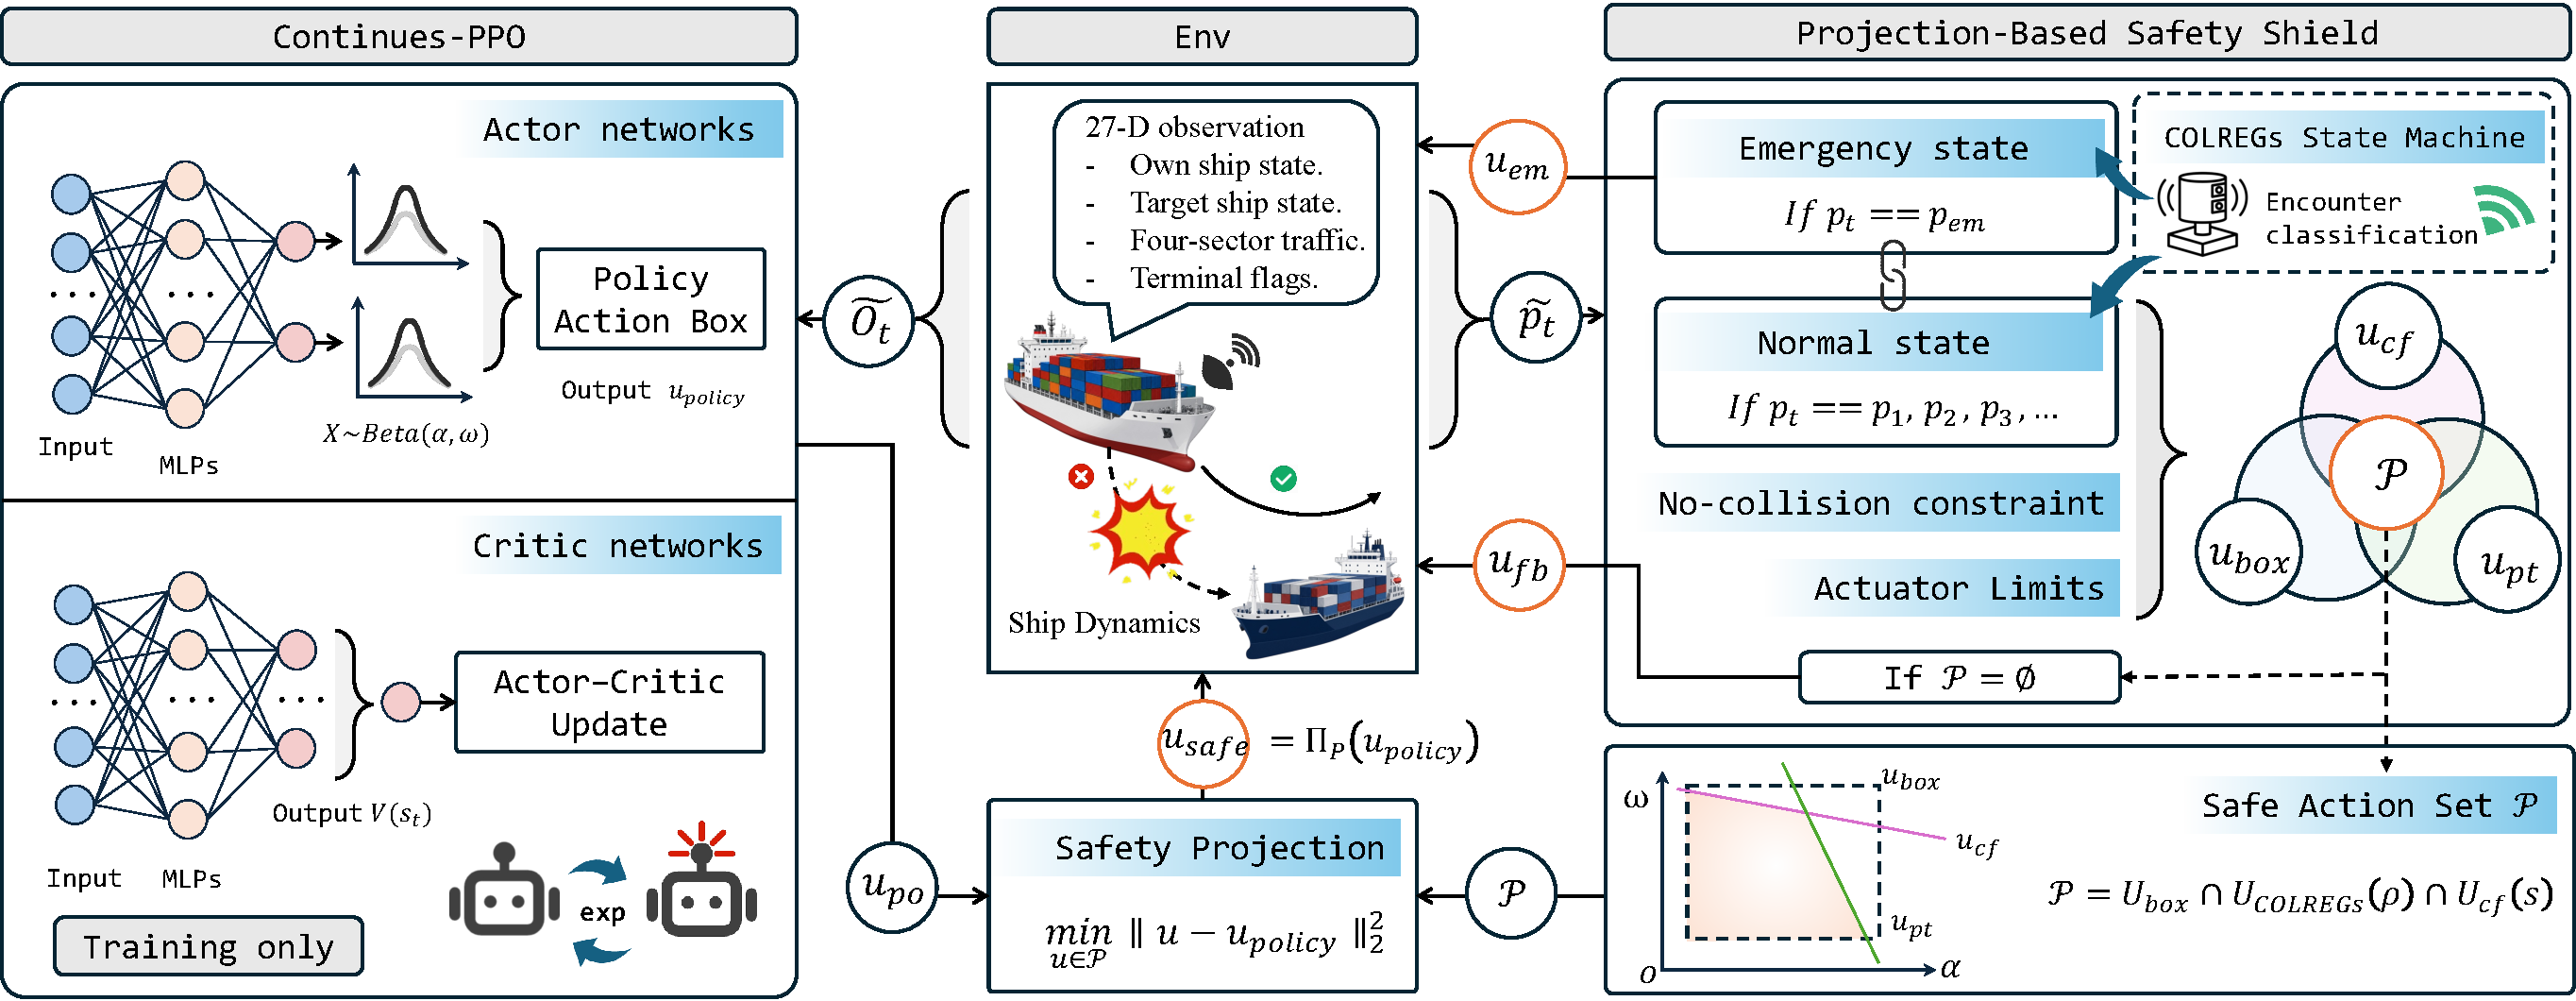
\includegraphics[width=\linewidth]{figs/fig1_overview.pdf}
 \caption{Overview of the method. \capnote{A $27$-dimensional observation enters the policy
 network, which emits a desired control command $u_{\mathrm{policy}}$ from a Beta
 distribution with bounded support. The rule state machine assigns the encounter to one of
 six situations. The safe control set $U_{\mathrm{safe}}$ is the intersection of the actuator
 limits, the half-plane of compliant directions, and the one-step collision-free constraint.
 A quadratic program projects $u_{\mathrm{policy}}$ onto $u_{\mathrm{safe}}$, which is then
 passed to the environment. The projection is part of the environment transition, so the
 shield sits inside the training loop. The two bypasses are exclusive. An emergency situation
 goes straight to the emergency controller, and every other situation falls back only when
 $U_{\mathrm{safe}}$ is empty. The panel at the lower right sketches the three constraint sets
 in the control plane.}}
 \label{fig:overview}
\end{figure}
%------------------------------------------------------------------------------



\noindent\textbf{A note on the guarantees.}\ Each proposition below is placed after the mechanism it applies to, and is given as a
statement, its assumptions, a proof sketch, and its scope. The scope paragraph names the
cases it does not cover.

\subsection{COLREGs Obligations as Half-Plane Constraints}
\label{sec:rulesets}

The rule state machine sorts the current encounter into six situations,
\begin{equation*}
\rho\in\{\rho_0\ \text{conflict-free},\ \rho_1\ \text{stand-on},\ \rho_2\ \text{head-on},\
\rho_3\ \text{crossing},\ \rho_4\ \text{overtaking},\ \rho_5\ \text{emergency}\},
\end{equation*}
and the decision is a conjunction of three groups of conditions. Each condition is a
predicate, that is, a named test on the two states that returns true or false.

The first group is the bearing sector, taken along the sidelight boundaries of the
convention. The second group is the heading relation, which separates nearly anti-parallel
from nearly parallel headings. The third group is collision possibility. It has two
parts. The speed set of the own vessel must intersect the collision cone of the target
vessel. The relative speed must also close the current center distance in time. The forward sector
has a half-angle of $5^\circ$ and the side sectors end at $112.5^\circ$. The overtaking band
has a half-angle of $67.5^\circ$. The occupancy of the target vessel is inflated by three
times its length, and the check horizon is $420$~s.

Four situations carry an obligation. More than one of their predicates can hold at the same
instant, so the four are tested in a fixed priority order and the first match wins. The
rows below are written in that priority order, which is not the order of the indices,
\begin{equation}
\begin{aligned}
\rho_2\ \text{head-on}&:\quad \mathrm{CP}\wedge\mathrm{Fr}(s_e,s_m)\wedge\mathrm{Ap},\\
\rho_3\ \text{crossing}&:\quad \mathrm{CP}\wedge\mathrm{Ri}(s_e,s_m)\wedge\mathrm{Tl},\\
\rho_4\ \text{overtaking}&:\quad \mathrm{CP}\wedge\mathrm{Be}(s_m,s_e)\wedge(v_e>v_m)\wedge\mathrm{Sd},\\
\rho_1\ \text{stand-on}&:\quad \bigl[\mathrm{CP}\wedge\mathrm{Le}(s_e,s_m)\wedge\mathrm{Tr}\bigr]\ \vee\ \rho_4(s_m,s_e),
\end{aligned}
\label{eq:situations}
\end{equation}
and all other cases fall into $\rho_0$. Stand-on is tested last, and its definition reuses
the overtaking predicate with the two vessels exchanged. Overtaking and being overtaken
swap the two vessel arguments, because overtaking places the own vessel in the aft sector
of the target vessel. The indices $\rho_0$ to $\rho_5$ are identifiers rather than a
ranking.

Entry into a give-way situation has two parts. A give-way predicate must not hold now. It must hold at every decision step of a $60$~s reaction window under constant-velocity extrapolation. The first part separates ``about to hold'' from ``already holds'', and it creates one asymmetry that Section~\ref{sec:sym} treats. The emergency situation is
entered by a stronger set-based prediction with a horizon of $180$~s.

\noindent\textbf{Compliant control set.}\ Each situation maps to an explicit constraint set
on the command,
\begin{equation}
 U_{\mathrm{colregs}}(\rho)=
 \begin{cases}
  U_{\mathrm{box}}, & \rho=\rho_0,\\[2pt]
  \{|a|\le\varepsilon_a\}\cap\{|\omega|\le\varepsilon_\omega\}, & \rho=\rho_1,\\[2pt]
  \{\omega\le-\omega_{\mathrm{turn}}\}, & \rho\in\{\rho_2,\rho_3\},\\[2pt]
  \{\omega\le-\omega_{\mathrm{turn}}\}\ \text{or}\ \{\omega\ge+\omega_{\mathrm{turn}}\}, & \rho=\rho_4,\\[2pt]
  U_{\mathrm{box}}, & \rho=\rho_5.
 \end{cases}
 \label{eq:ucolregs}
\end{equation}
Head-on and crossing require a turn to starboard. Overtaking allows a turn to either side.
Stand-on holds course and speed. Each set is a half-plane or an interval on the plane of control commands. A set of this shape can be entered by projection, so the commands never have to be enumerated.

\noindent\textbf{Quantifying a readily apparent action.}\ The convention asks a give-way
action to be large enough to be seen in time. We quantify this as a course change of at
least a given threshold within the maneuver window. With a window of $40$~s and a threshold
of $20^\circ$,
\begin{equation}
 \omega_{\mathrm{turn}}=\frac{\Delta_{\mathrm{lt}}}{T_M}=\frac{20^\circ}{40~\mathrm{s}}\approx 0.008727~\mathrm{rad/s}.
 \label{eq:omegaturn}
\end{equation}
This is the smallest compliant turn rate. Any turn at least this large complies, and
the bound cannot be lowered.

The predicate structure and the numerical thresholds follow the temporal-logic
formalization of the maritime rules \citl{krasowski2024}{Krasowski and Althoff 2024}. Three
details are settled here. The inflation radius and the half-width of the speed set are
stated explicitly. Entry into a give-way situation is made symmetric
(Section~\ref{sec:sym}). The predicate set is then mapped to a constraint set on continuous
commands.


\subsection{Safe Control Set and Projection}
\label{sec:proj}

\subsubsection{One-Step Collision-Free Constraint}
\label{sec:collfree}

At each decision step the applied command must keep the two hulls apart at the end of the
next step. Written directly, that condition is not convex. We replace it by a convex subset of itself, built in three steps.

First, the occupancy of the target vessel after one step is over-approximated by a disk.
The center follows a constant-velocity extrapolation, and the radius includes a safety margin. The own vessel is over-approximated by its circumscribed circle. The two hulls then stay apart whenever the center distance is at least the sum of the two radii, written $d_{\mathrm{safe}}$.

Second, let $n$ be the unit vector from the target vessel to the nominal end point of the
own vessel, and let $\delta$ be that distance. The end point follows from the policy command clipped to the action box.

Third, the end point is expanded to first order in the command,
$p_e(u)\approx p_{\mathrm{nom}}+J(u-u_{\mathrm{nom}})$. The end point must lie on the safe
side of the separating hyperplane. This gives one linear inequality in the command:
\begin{equation}
 \underbrace{-\,n^{\!\top}\!J}_{\textstyle g^{\!\top}}\,u\ \le\
 \underbrace{-\bigl(d_{\mathrm{safe}}-\delta+n^{\!\top}\!J\,u_{\mathrm{nom}}\bigr)}_{\textstyle h},
 \qquad U_{\mathrm{cf}}(s)=\{u: g^{\!\top}u\le h\}.
 \label{eq:ucf}
\end{equation}

A first-order expansion is neither an inner nor an outer approximation. The sign of the
remainder changes with the curvature. Equation~\eqref{eq:ucf} alone therefore does not
establish conservatism. The margin inside the safety distance is what does. With that margin the constraint acts at a center distance of $590$--$840$~m, with a median of $714$~m over this library. Hull contact needs a much smaller distance. The margin absorbs the linearization residual. The cost is a tighter constraint that rejects some commands which are in fact safe.

The linearization holds only locally. In the far field a sufficient condition is available that does not rely on it.

\begin{prop}[One-step collision freedom in the far field]\label{prop:farfield}
Let $d$ be the center distance between the own vessel and a single target vessel. If
\begin{equation}
 d \;\ge\; d_{\mathrm{safe}} + v_{\mathrm{obs,max}}\Delta t + \rho_{\mathrm{ego}},
 \label{eq:farfield}
\end{equation}
then the two conservative circumscribed occupancies do not intersect after one decision
step. Here $d_{\mathrm{safe}}$ is the sum of the two circumscribed radii, and
$\rho_{\mathrm{ego}}$ is the largest displacement of the own vessel in one step.
\end{prop}

\noindent\textbf{Assumptions.}\ A single target vessel. The speed of the target vessel is
at most $9.5$~m/s. That bound is not implied by the dynamics and is stated separately; the
largest value measured over the $2{,}000$ scenarios of the library is $7.10$~m/s. The
target vessel holds its speed within the step.

\noindent\textbf{Proof sketch.}\ By the triangle inequality, the center distance after the
step is at least $d$ minus the one-step displacement bound of each vessel. It is therefore
at least $d_{\mathrm{safe}}$.

\noindent\textbf{Scope.}\ The triangle inequality does not depend on direction, so a
head-on encounter is the worst case. With the constants of this library the threshold is
about $764$~m. The statement covers one step. It does not extend to the steps after it, and
it does not cover the near field.

\subsubsection{Projection as a Quadratic Program}

The safe control set is the intersection of three sets,
\begin{equation}
 U_{\mathrm{safe}}(s,\rho)=U_{\mathrm{box}}\cap U_{\mathrm{colregs}}(\rho)\cap U_{\mathrm{cf}}(s),
 \label{eq:safeset}
\end{equation}
and it is a convex polygon in $\mathbb{R}^2$. The applied command is the Euclidean
projection of the policy command onto that set,
\begin{equation}
 u_{\mathrm{safe}}=\Pi_{U_{\mathrm{safe}}}(u_{\mathrm{policy}})
 =\arg\min_{u\in U_{\mathrm{safe}}}\lVert u-u_{\mathrm{policy}}\rVert_2^2 .
 \label{eq:qp}
\end{equation}

The feasible set is an intersection of half-planes, so it can be written as $U_{\mathrm{safe}}=\{u:Au\le b\}$. The first four rows are the action box, the fifth is the compliant-direction half-plane, and the sixth is the collision-free constraint of Equation~\eqref{eq:ucf}. The program has two variables and at most six constraints. It is small enough to solve online at every decision step.



\begin{prop}[Directional compliance on every give-way step]\label{prop:comply}
Consider any decision step that the rule state machine assigns to a give-way situation and
on which the projection is feasible. The applied command $u_{\mathrm{safe}}$ then lies in
the compliant-direction half-plane.
\end{prop}

\noindent\textbf{Assumptions.}\ A single target vessel, and a correct decision by the state
machine. The second assumption inherits one conservative bias of the collision-possibility
predicate. That predicate uses the center distance, and it can miss a trailing encounter in
which the two speeds are close.

\noindent\textbf{Proof sketch.}\ The compliant half-plane enters the quadratic program as a
hard constraint. Any feasible point satisfies it, and the projection returns a feasible
point. The statement holds by construction. It does not depend on the training outcome or
on the random seed.

\noindent\textbf{Scope.}\ Emergency situations are not covered, because their branch
bypasses the compliance constraint by design. Steps on which the safe control set is empty
and the fallback is used are not covered either.

\subsubsection{Fallback and the Unavoidable-Collision Criterion}
\label{sec:fallback}

When the safe control set is empty, the projection has no solution. A substitute rule then
supplies the command. We call it the fallback, and it carries no guarantee. The fallback
branches on the encounter situation. It does not try a fixed list of options in order. The
two branches below are mutually exclusive.

\noindent\textbf{Emergency branch.}\ An emergency situation takes a separate path. No
collision-free constraint is built, and Equation~\eqref{eq:qp} is not solved. A stateful
geometric controller supplies the command instead, and its lifetime is one emergency event.
It has three modes. A near head-on approach ahead tracks a lateral point fixed at the
onset of the emergency. A target vessel astern that acceleration can clear takes a
straight-line escape inside the reaction window. Every other case tracks a point that
moves with the target vessel. One position-tracking law turns all three into a control
command. This controller offers no guarantee. Its purpose is a
defined behavior once no compliant feasible command remains.

\noindent\textbf{Other situations.}\ Outside an emergency situation the fallback is used
only when the safe control set is empty. A degenerate case is tested first. If the
linearization gives no usable separation direction, the command is projected onto the action
box alone. Otherwise the direction constraint is relaxed, and the collision risk is
minimized if that also fails. The last two branches solve on the actuator limits and drop
the compliance constraint as a whole. The turn rate can then leave the policy action box, so
saturation is reported against each box separately.

These branches almost never fire on this scenario library. With course and speed held,
the median closest center distance is about $1{,}300$~m, so the safe control set is
rarely empty. Purpose-built conflict cases exercise the branches, and their outcome is
reported with the shield measurements.

The emergency branch offers no guarantee. It can still decide whether the situation was
already beyond recovery.

\begin{prop}[Conservative criterion for an unavoidable collision]\label{prop:imminent}
Consider a single target vessel at constant velocity. Let $R_{\mathrm{box}}(t)$ be an
over-approximation of the reachable centers of the own vessel, and let $O(t)$ be the hull
rectangle of the target vessel. If
\begin{equation}
 \exists\,t^\ast\in[0,T]:\quad R_{\mathrm{box}}(t^\ast)\subseteq\bigl(O(t^\ast)\oplus\mathrm{disk}(r_{\mathrm{insc}})\bigr),
 \label{eq:imminent}
\end{equation}
then the collision is unavoidable, and every feasible control sequence meets that target
vessel at $t^\ast$.
\end{prop}

\noindent\textbf{Assumptions.}\ A single target vessel at constant velocity. The hull size
of the target vessel must not be overstated, since a beam larger than the true value makes
the test unreliable. The horizon is $120$~s, evaluated at $241$ equally spaced instants.

\noindent\textbf{Proof sketch.}\ The rate of change of the velocity vector is bounded. A
double integration gives the two semi-axes of $R_{\mathrm{box}}$, which therefore
over-approximates the true reachable centers. The inscribed circle under-approximates the
hull. Once every reachable center lies inside the inflated occupancy of the target vessel,
no control command can avoid contact.

\noindent\textbf{Scope.}\ The criterion is one-sided. It can miss a case, and it never
raises a false alarm. A negative result therefore does not mean that the collision is
avoidable. The criterion also acts late rather than early, and maneuvering target vessels
are not covered. On $20{,}000$ random scenarios and $735$ selected scenarios it produced no false
positive. After the envelope was hardened, $1{,}500$ further fuzz cases produced none
either.


\subsection{Shielded Policy Optimization}
\label{sec:rl}

The shield is not applied after the policy as a post hoc correction. The projection of
Equation~\eqref{eq:qp} is placed inside the environment transition. The policy emits
$u_{\mathrm{policy}}$, the environment applies $u_{\mathrm{safe}}$, and it returns the
successor state and the reward. The policy therefore faces the composed transition
\begin{equation}
 s_{t+1}\ \sim\ P\bigl(\,\cdot\,\bigm|\, s_t,\ \Pi_{U_{\mathrm{safe}}(s_t,\rho_t)}(u_t)\bigr),
 \qquad u_t\sim\pi(\cdot\mid s_t),
 \label{eq:shielded-mdp}
\end{equation}
rather than the $P(\cdot\mid s_t,u_t)$ of a post hoc filter. The policy learns on the
transition it will actually meet, so it adapts to the projection during training instead of
meeting an unfamiliar filter afterwards.

\noindent\textbf{Learning algorithm.}\ All configurations are trained with proximal policy
optimization \citl{schulman2017}{Schulman et al. 2017}. The continuous-action
configurations use its standard form. The discrete-action baselines use its maskable
variant, because action masking is what makes a discrete shield possible. Both action
spaces therefore share one policy-gradient algorithm, which removes a source of difference
between them. The masking itself remains a difference, and it is intrinsic to the discrete
method rather than a choice made here.

\subsubsection{Reward Function}

The reward is a sum of five terms,
\begin{equation}
 r=r_{\mathrm{sparse}}+r_{\mathrm{goal}}+r_{\mathrm{velocity}}+r_{\mathrm{deviate}}+r_{\mathrm{colregs}}.
 \label{eq:reward}
\end{equation}
A sparse terminal term scores arrival, timeout, stalling and collision, and charges a
fixed penalty for every step under emergency control. A dense approach term rewards the
change in distance to the goal over one step. A speed term penalizes speed outside the
cruise band $[2.5,\,8.0]$~m/s. A cross-track term penalizes lateral deviation from the
start-to-goal line and saturates at $2{,}000$~m. A soft compliance term decays with
distance. It is active only in the reward-shaping baseline and in the discrete
configurations. Every continuous configuration here sets it to zero, because compliance is
carried by the hard constraint of Equation~\eqref{eq:ucolregs}.

The five terms are taken from \citl{krasowski2024}{Krasowski and Althoff 2024}, with three
declared deviations. The approach term uses the difference of distances between two
steps. The soft compliance term is rescaled, because its original calibration sits at a
scale about fifty times smaller than these scenarios. One clause of the
emergency-release test is read by its physical meaning rather than its literal sign,
since the two disagree.

\subsubsection{Bounded Action Distribution}

A continuous policy usually emits an unbounded Gaussian and clips the sample to the
action box. That conflicts with Equation~\eqref{eq:qp} for two reasons, both from the
clipping. First, common implementations feed the clipped action to the environment and
the unclipped action to the policy gradient. Once the mean leaves the box, moving
further out changes no reward, the
gradient reaches a plateau, and any penalty on action smoothness loses its grip. Second, the differential entropy of a Gaussian has no upper bound while the entropy
coefficient is a constant. The standard deviation therefore has a one-way channel to
grow, which pushes still more samples outside the box.

We use a Beta distribution with support on a closed interval. Actions can then never leave
the box, clipping becomes the identity map, both channels close, the smoothness penalty is
differentiable everywhere, and the entropy is bounded above. The network emits two reals
per control axis, and
\begin{equation}
 \alpha=\mathrm{softplus}(\tilde\alpha)+1,\quad \beta=\mathrm{softplus}(\tilde\beta)+1,\qquad
 u=u_{\mathrm{lo}}+(u_{\mathrm{hi}}-u_{\mathrm{lo}})\,z,\quad z\sim\mathrm{Beta}(\alpha,\beta)
 \label{eq:beta}
\end{equation}
gives the shape parameters and the applied action. Evaluation uses the mode instead of a
sample. The offset of one keeps both shape parameters above unity, and that constraint
cannot be dropped. Below unity the Beta density is U-shaped and diverges at the two ends,
and the mode then sits at an endpoint. Because evaluation always takes the mode, such a
policy would silently corrupt every reported number, and the aggregate metrics would give
no sign of it.

\subsubsection{Symmetric Entry into Give-Way Situations}
\label{sec:sym}

In the state machine, entry into a give-way situation is not symmetric. From the
conflict-free situation it is triggered only by the persistence condition. From the
stand-on situation a separate immediate condition also applies. We add the symmetric
branch. When the persistence condition
does not fire, the immediate condition is checked, and the give-way situation is entered if
it already holds. The obligation is then recognized at the same moment on both routes. The
change alters the command that the shield applies, so training and evaluation must use the
same setting.

A purpose-built case shows why the branch is needed. Suppose an encounter already satisfies
a give-way predicate at the initial instant. The clause ``does not hold now'' can then never
be satisfied. The persistence condition never fires, and the encounter is never recognized
as a give-way situation. On a set of such adversarial cases the persistence route alone
gives $0$ give-way decision steps. With the immediate branch it gives $201$. These cases are
synthetic and illustrate the mechanism, so they are reported apart from the main results.

\subsubsection{Training Setup}
\label{sec:train}

Apart from the entropy coefficient, which is set to $0.01$, and the bounded action
distribution, every hyperparameter takes the default of the implementation library and is
left untuned. The libraries are Stable-Baselines3 2.3.2
\citl{raffin2021}{Raffin et al. 2021} and sb3-contrib 2.3.0, and the advantage is computed
by generalized advantage estimation \citl{schulman2016}{Schulman et al. 2016}. The discrete
and continuous configurations agree on every one of these values, so the hyperparameters are
not a source of difference between them. Running normalization of the observation and the
reward is not optional. Without it the large-scale approach term in
Equation~\eqref{eq:reward} drives the policy to a degenerate solution that holds station.


%==============================================================================
% §5 实验 —— 对应中文稿 657–905 行
%   🔴 相对中文稿的取舍（登记在 `英文写作规范.md §九`）：
%      · 砍掉算法框 alg:score（离线评分器）—— 一个 float 约 1/3 页，规则四句话说得清；
%      · 表 tab:arms 压掉「相对上一级只改」一列，改写进表注（那列每格都是长句）。
%   🔴 \prov{...} 里的数字全部是**验证集 100 场景的暂用值**，重评到手后整批替换。
%==============================================================================
\section{Experiments}
\label{sec:exp}

\subsection{Scenarios and Configurations}
\label{sec:setup}

The experiments use the two-vessel encounter library of the CommonOcean benchmark
\citl{krasowski2022}{Krasowski and Althoff 2022}, which holds $2{,}000$ scenarios. Each
scenario fixes the initial pose and speed of the controlled vessel. It also fixes the
initial state and the planned track of the target vessel. It ends with a goal region that
has a position gate, a heading gate, and a time limit. The encounter geometry is generated programmatically over a range
of relative bearings, crossing angles, and closing speeds. Target vessels are $200$ to
$300$~m long, and an episode lasts at most $170$ decision steps.

Classifying the library by the geometric predicates returns crossing and head-on only.
\textbf{The library contains no overtaking scenario}, and the official test set holds $395$
crossing and $205$ head-on cases. The overtaking branch of Equation~\eqref{eq:ucolregs}
therefore cannot be tested empirically here. The conclusions state this.

The official split of $1{,}400$ training and $600$ test scenarios is used. The training side
is split again into $1{,}300$ for training and $100$ for validation. The validation set is
used only for monitoring during training and for selecting a checkpoint. The test set is
never accessed during training or tuning. An independent recount confirmed that the two sets
are disjoint, so the evaluation sample size is $600$.

Table~\ref{tab:arms} lists nine configurations. They form one connected ladder, and each
level changes a single variable from the level before it. The contribution of each mechanism
can therefore be read on its own.

%------------------------------------------------------------------------------
\begin{table}[htbp]
 \caption{The nine configurations}
 \label{tab:arms}
 \centering\small
 \setlength{\tabcolsep}{3pt}
 \begin{tabular*}{\linewidth}{@{\extracolsep{\fill}}l ccccccc@{}}
  \toprule
  Configuration & Cont. & Shield & Masking & Soft rew. & Shaping & Bounded & Sym. entry \\
  \midrule
  Discrete baseline        & $\times$ & $\times$ & $\times$ & $\times$ & $\times$ & - & - \\
  Discrete, soft reward    & $\times$ & $\times$ & $\times$ & $\checkmark$ & $\times$ & - & - \\
  Discrete, masking        & $\times$ & $\times$ & $\checkmark$ & $\checkmark$ & $\times$ & - & $\times$ \\
  Continuous, no shield    & $\checkmark$ & $\times$ & $\times$ & $\times$ & $\times$ & $\times$ & $\times$ \\
  Continuous, shield       & $\checkmark$ & $\checkmark$ & $\times$ & $\times$ & $\times$ & $\times$ & $\times$ \\
  Ablation reference       & $\checkmark$ & $\checkmark$ & $\times$ & $\times$ & $\checkmark$ & $\times$ & $\times$ \\
  Ablation, bounded only   & $\checkmark$ & $\checkmark$ & $\times$ & $\times$ & $\checkmark$ & $\checkmark$ & $\times$ \\
  Ablation, symmetric only & $\checkmark$ & $\checkmark$ & $\times$ & $\times$ & $\checkmark$ & $\times$ & $\checkmark$ \\
  Ours                     & $\checkmark$ & $\checkmark$ & $\times$ & $\times$ & $\checkmark$ & $\checkmark$ & $\checkmark$ \\
  \bottomrule
 \end{tabular*}

 \vspace{4pt}
 \begin{minipage}{\linewidth}\small
 \textbf{Notes.} A check mark is on, a cross is off, and a dash is not applicable. Rows run
 from the discrete baseline to Ours. Three steps of the ladder carry a companion
 variable that cannot be separated. The action space changes together with the policy
 distribution, the continuous-only shaping is a bundle of four items, and the bounded
 distribution also changes the initial exploration scale. Those three steps can only be
 attributed as a whole.
 \end{minipage}
\end{table}
%------------------------------------------------------------------------------

\noindent\textbf{What the unshielded continuous configuration can show.}\ A
continuous-action configuration without a shield can only take the plainest form, namely an
unbounded Gaussian, an asymmetric give-way entry, and no shaping. Giving it the
continuous-only shaping would break the symmetry with the discrete baseline and the
attribution would fail. The unbounded Gaussian also pushes many samples past the action
box. In a small re-evaluation during the exploration phase, which is not the setting of
the formal experiment, about $73\%$ of the decision steps of that policy sat against the
boundary. The gain attributed to the shield is therefore measured against
the weakest form of continuous action. For the same reason the step from the discrete
baseline to that configuration can be negative, and it should be read as a conservative
lower bound.

\subsection{Metrics and Evaluation Protocol}
\label{sec:metrics}

\noindent\textbf{Metrics.}\ The main metrics are the arrival rate, the collision rate, the COLREGs violations per
episode, the share of steps under emergency control, and the episode duration. The
violation count is split into give-way and stand-on violations. Control quality, safety
margin, shield behavior and the single-step solve time are also reported, and every
metric is broken down by encounter situation. The reward function differs across configurations, so the
episode return is never compared across them.

\noindent\textbf{How violations are counted.}\ Violations do not come from the situation
decision of the shield. An offline scorer that sees only the trajectory re-decides at each step, from the bare
situation predicates, whether the own vessel is under a stand-on or a give-way
obligation. A stand-on
violation is counted per step, once the signed heading change accumulated over the
obligation period exceeds the stand-on tolerance, and the accumulator is reset when the
obligation ends. A give-way violation is counted per encounter, and an encounter counts as
a violation only when no turn in the required direction ever reaches the readily apparent
threshold. The scorer applies one rule to this method and to every baseline, including the
geometric controllers that have no state machine, so the comparison is made under one
condition.

\noindent\textbf{The counting window and the shield do not coincide.}\ The scorer
accumulates the heading change over a whole obligation period, while the shield constrains
the change inside a single maneuver window. The two windows differ in length. Emergency situations and fallback steps also bypass
the constraint by design. The shield therefore does not guarantee a violation count of zero, and this paper
does not claim one. In particular, Proposition~\ref{prop:comply} guarantees the turn
direction on every give-way step. It does \textbf{not} imply a give-way violation count of
zero. How often the mismatch occurs was not measured.

\noindent\textbf{Training budget.}\ Each configuration is trained with $8$ random seeds, one
run per seed. The $72$ runs together cover about $730$ million environment steps. The
scenario split is fixed by a separate seed, so every run sees the same scenarios. Every configuration inside one
table is evaluated on one machine in one pass, so that machine differences do not enter the
evaluation. Machine time did not allow the same during training. For $5$ of the $8$ seeds
all configurations were trained on one machine, and the other $3$ seeds are spread over two
or three machines. Those machines run the same image and the same training code, with a
byte-identical fingerprint of the training path, and with the thread count locked to one.
\textbf{No bit-level cross-machine check was run on this batch, so machine differences are
not excluded. This is listed as a limitation.}

\noindent\textbf{Checkpoint selection.}\ Twenty checkpoints are saved per run at even
intervals, and each is evaluated once on the validation set. The selection rule was fixed in
advance and has no tunable part. The candidates are those twenty checkpoints, the criterion
is the highest arrival rate on the validation set, ties go to the earlier checkpoint, and
the test set is never touched.
\textbf{The rule is itself biased, so two versions are reported.} The validation set holds
only $100$ scenarios, and the binomial standard error of the arrival rate is about $4$
points. Taking the maximum over $20$ candidates lifts the reported value by about $7.5$
points in expectation. That is four times the drift of about $1.6$ points that the
same-machine rule was written to prevent. The best-checkpoint version and the
last-checkpoint version are therefore both reported.

\noindent\textbf{Reading the figures.}\ Figures~\ref{fig:tradeoff} and~\ref{fig:ablation}
are computed on the same test set as Table~\ref{tab:main}. Figures~\ref{fig:curves}
and~\ref{fig:shield} are recorded during training and are labelled as such. Violation counts
in the figures are the sum of stand-on and give-way violations.

\noindent\textbf{Statistics.}\ The paired test is a per-seed paired sign test, whose smallest two-sided value with $8$
seeds is $p=2/2^{8}=0.0078$. Error bars are bootstrap $95\%$ intervals resampled over
seeds. A run counts as converged when its arrival rate on the validation set reaches
$50\%$. Diverged seeds are counted in the main table as they are, and a
converged-seeds-only version is also reported.

\subsection{Main Comparison}
\label{sec:res-main}

%------------------------------------------------------------------------------
\begin{table}[htbp]
 \caption{Main comparison, all seeds. \capnote{Official test set, $N=600$, at the
 checkpoint selected on the validation set.}}
 \label{tab:main}
 \centering\small
 \setlength{\tabcolsep}{4pt}
 \begin{tabular*}{\linewidth}{@{\extracolsep{\fill}}lcccccccc@{}}
  \toprule
  Configuration & $n$ & Conv. & Arrival \% [CI] & Coll. \% & Viol./ep. & Turn $\Delta$ & Thr. $\Delta$ & Emerg. \% \\
  \midrule
  Discrete baseline         & 8 & \textbf{8/8} & 97.8 [97,\,98] & 2.00 & 3.04 & 0.0149 & 0.0160 & 0.00 \\
  Discrete, soft reward     & 8 & 7/8 & \textbf{98.2 [97,\,98]} & 1.58 & 2.95 & 0.0141 & 0.0169 & 0.00 \\
  Discrete, masking         & 8 & 6/8 & 93.3 [10,\,96] & 0.08 & 1.16 & 0.0112 & 0.0205 & 4.64 \\
  Continuous, no shield     & 8 & 7/8 & 98.0 [96,\,99] & 1.25 & 4.44 & 0.0267 & 0.0106 & 0.00 \\
  Continuous, shield        & 8 & 5/8 & 69.0 [16,\,91] & 0.17 & 1.02 & 0.0246 & 0.0158 & 2.86 \\
  Ablation reference        & 8 & 5/8 & 84.5 [9,\,90] & 0.33 & 1.13 & 0.0140 & 0.0059 & 3.36 \\
  Ablation, bounded only    & 8 & 7/8 & 90.8 [66,\,92] & 0.17 & 0.67 & 0.0049 & 0.0076 & 2.27 \\
  Ablation, symmetric only  & 8 & 6/8 & 75.5 [4,\,89] & \textbf{0.00} & 0.82 & 0.0167 & 0.0053 & 2.61 \\
  Ours                      & 8 & \textbf{8/8} & 88.2 [84,\,90] & \textbf{0.00} & \textbf{0.53} & 0.0054 & 0.0078 & 2.42 \\
  \bottomrule
 \end{tabular*}

 \vspace{4pt}
 \begin{minipage}{\linewidth}\small
 \textbf{Notes.} The best value in each column is in bold. The turn and throttle increment
 columns are \textbf{not} marked, because they cannot be compared across action spaces
 (Section~\ref{sec:train}). The share of emergency steps is descriptive and is neither good
 nor bad.
 \end{minipage}
\end{table}
%------------------------------------------------------------------------------

Three readings follow from Table~\ref{tab:main}. First, Ours has the lowest violation count
per episode of all nine configurations, at $0.53$, against $1.16$ for the discrete safe
baseline and $4.44$ for the unshielded continuous configuration. A per-seed paired sign test
gives $8$ wins out of $8$ against every other configuration except the two shielded
ablations, at $p=0.0078$. Second, Ours is the only shielded configuration that reaches the
convergence criterion on all $8$ seeds. Third, the arrival rate of Ours is $88.2\%$, which
is below the three unshielded configurations and below the discrete safe baseline. That gap
is the cost of the shield and it is not claimed as a benefit anywhere in this paper.
Table~\ref{tab:main} is also reported in a converged-seeds-only version, because a diverged
seed pollutes the per-episode averages and the direction of that pollution differs by
configuration. Per-seed raw values accompany the table.

\begin{figure}[htbp]
 \centering
 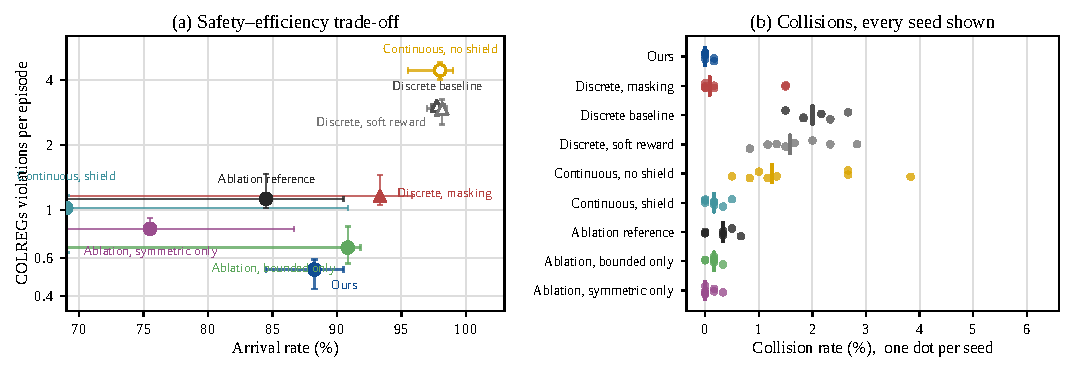
\includegraphics[width=\linewidth]{figs/fig2_tradeoff.pdf}
 \caption{Safety and efficiency. \capnote{Official test set, the same source as
 Table~\ref{tab:main}. Points are medians across seeds and error bars are bootstrap $95\%$
 intervals resampled over seeds. Circles are continuous action spaces, triangles are discrete
 ones, and filled markers carry a shield. The lower right of panel (a) is the ideal region.
 The bars are wide because several configurations contain a diverged seed.}}
 \label{fig:tradeoff}
\end{figure}

\subsection{Ablation Study}
\label{sec:res-ablation}

The four ablation configurations form a complete $2\times2$ design over the bounded action
distribution and the give-way entry. Everything else is identical, and the comparison is
paired by seed. The bounded distribution lowers the median turn increment by $65\%$, with
all $8$ seeds moving in the same direction and a paired signed-rank value of $p=0.008$. It
lowers the violations per episode by $41\%$, again $8$ of $8$, with $p=0.008$. The symmetric
entry alone \textbf{raises} the turn increment by $19\%$, with $p=0.016$, and it lowers the
violations per episode by $27\%$, with $p=0.008$. With both changes on, the turn increment
falls by $61\%$ and the violations by $53\%$. Neither can be separated statistically from
the bounded distribution alone, at $p=0.74$ and $p=0.11$. The two changes therefore divide
the work. Smoothness comes entirely from the bounded action distribution, and both
contribute to compliance.

This group is the only place where the smoothness result can be read. All four
configurations run the same action-increment penalty, so the difference can be attributed
to the bounded action distribution rather than to an extra reward term. A comparison against
the discrete baseline would not be valid here, because that penalty applies to a quantity
the discrete configurations do not have. Adding the bounded distribution also carries a companion
variable, since the initial exploration scale differs by about a factor of $2.5$ on the
acceleration axis. A converged-seeds-only version is given for this group
as well.

\begin{figure}[htbp]
 \centering
 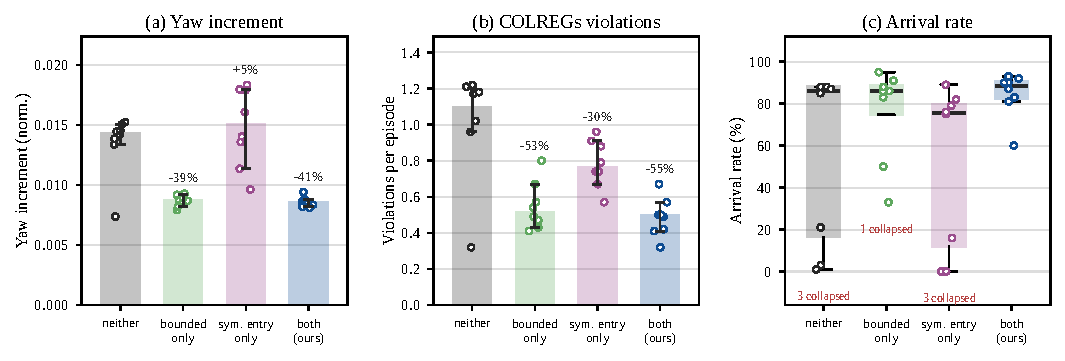
\includegraphics[width=\linewidth]{figs/fig3_ablation.pdf}
 \caption{The $2\times2$ ablation. \capnote{Paired by seed. Bars are medians across seeds,
 error bars are bootstrap $95\%$ intervals, and open points are single seeds. The label above
 each bar is the change relative to the leftmost bar. The paired tests are reported in the
 text. The arrival rate is bimodal, so it is drawn as a box plot and the number of diverged
 seeds is printed below each box.}}
 \label{fig:ablation}
\end{figure}

\subsection{Training Reliability and Sample Efficiency}
\label{sec:res-reliability}

Figure~\ref{fig:curves} is taken from training. It answers two questions that do not need
the re-evaluation, namely whether the shield costs learning speed, and how many seeds of
each configuration reach a working policy.

First, there is a cost, and it appears in learning speed. On the training scenarios the
unshielded discrete baseline reaches an arrival rate of $96\%$ by $2$ million steps. The
shielded continuous configuration is at $33\%$ at that point, and it reaches $88\%$ at the
end of training. The shielded discrete baseline lies between the two, at $51\%$ and $93\%$
(Figure~\ref{fig:curves}b). Panels (c) and (d) give what is bought. The unshielded
configurations hold a collision rate near $1.8\%$ throughout training and more than
$2.4$ violations per episode. The shielded configurations sit at a collision rate of zero
and near $0.5$ violations per episode. The shield removes risk from the outcome,
and it narrows the exploration space at the same time. Slower learning is the direct
consequence of that narrowing.

Second, reliability differs a great deal among the shielded configurations. Under the
convergence rule declared in advance, all $8$ seeds of Ours reach a working policy, and it
is the only shielded configuration for which this holds. The shielded ablation
configurations reach $5$ to $7$ seeds, and the discrete safe baseline reaches $6$
(Figure~\ref{fig:curves}e). The two changes therefore improve more than the final numbers.
They also lower the chance that training itself fails. Diverged seeds are counted as they
are, and a converged-seeds-only version is given.

\noindent\textbf{A counterexample that has to be stated.}\ On the test set of $600$, $23$ of
the $48$ shielded runs have a collision rate of exactly zero, and $25$ do not. The largest is
$1.50\%$, on two seeds of the discrete safe baseline. For Ours, $6$ of the $8$ seeds have no
collision at all and the other two have exactly one collision each, which is $0.17\%$. The
earlier figure of zero came from the validation set of $100$ scenarios, where a single
collision is below the resolution of the sample. This agrees with the scope statements of
Section~\ref{sec:method}. The guarantees by construction cover one-step collision freedom in
the far field and the turn direction on give-way steps. They do not cover emergency
situations or the fallback. A collision rate of zero is therefore an observation and not a
guarantee.

\begin{figure}[htbp]
 \centering
 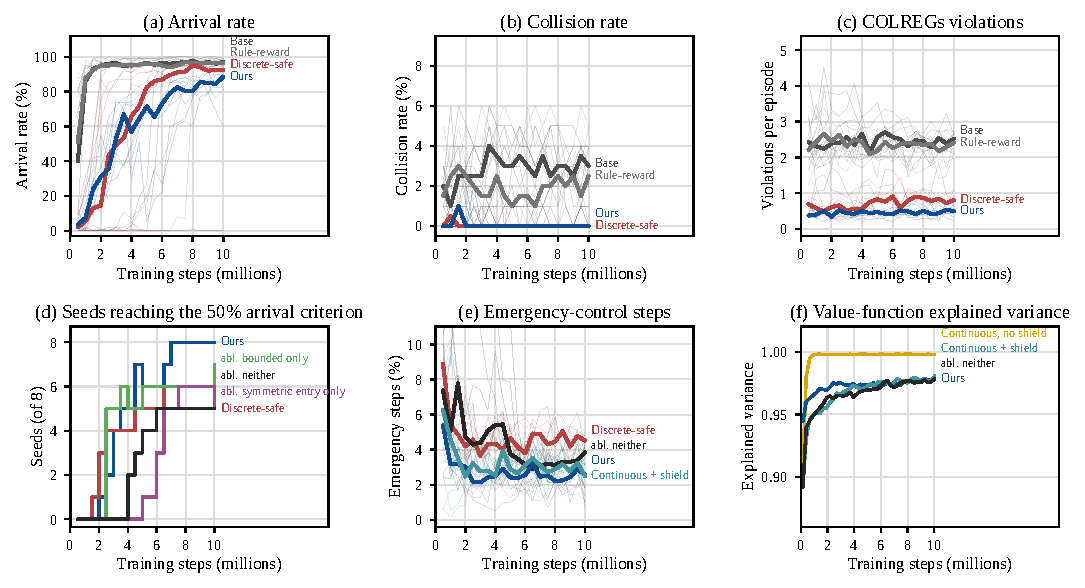
\includegraphics[width=\linewidth]{figs/fig4_training_reliability.pdf}
 \caption{Training curves. \capnote{Thick lines are medians and shaded bands are
 interquartile ranges over \textbf{converged seeds only}, because a diverged seed pulls the
 band to zero. The fraction in the legend is the number of converged seeds out of eight.
 Panels (a) to (c) and (f) are recorded once per rollout on the training scenarios, so they
 carry exploration noise. Panel (d) is measured on the validation set once per checkpoint,
 which is why it has fewer points. Panel (e) counts all eight seeds. \textbf{The reward
 function differs across configurations, so the level in panel (a) is not compared across
 them.}}}
 \label{fig:curves}
\end{figure}

\subsection{Behavior of the Safety Shield}
\label{sec:res-shield}

The emergency branch is the only part of this method with no guarantee, so its use is
reported separately. At the end of training,
the projection produced $93.6\%$ of the control commands. The emergency controller produced
$6.2\%$, and the three fallback branches produced $0.22\%$ in total
(Figure~\ref{fig:shield}a). On the test set the share of emergency steps is $2.42\%$, against $4.64\%$ for the
discrete safe baseline. The fallback is rare because it is used only when the safe
control set is empty, which seldom happens outside an emergency situation. Collisions are rare enough that their source cannot be attributed with confidence. Ours
records two collisions in $4{,}800$ test episodes. If a collision falls under emergency
control, then it occurs on a step where the last resort had already been engaged and had
failed. Those steps
lie outside the scope of Proposition~\ref{prop:farfield} by definition, since that
proposition covers the far field, non-emergency, single-step case. This is not a
counterexample to it, but it does confirm that the emergency branch is an empirical
fallback.

The size of the projection correction is normalized by the half-width of the action box.
At the end of training its median is $0.082$ and its interquartile range is
$[0.065,\,0.102]$. The gap between the command of the policy and what the rules require
therefore stays within about a tenth of the control range. It also narrows during training
(Figure~\ref{fig:shield}c). Among the four shielded continuous configurations the correction
is largest for the symmetric-only configuration, at $0.093$, and smallest for the
bounded-only configuration, at $0.066$. That ordering matches the turn increments in
Figure~\ref{fig:ablation}.

\noindent\textbf{Online cost.}\ The projection is one quadratic program with two variables and at most six constraints.
The timings below come from a single thread of the $32$-core Linux server that ran the
evaluation (\TBD), over $1{,}872$ decision steps of the trained policy. The median solve
time is $4.11$~ms and the $99$th percentile is $8.85$~ms. The forward pass of the policy
adds a median of $0.44$~ms. A whole decision step, including the environment, has a
median of $5.30$~ms and a $99$th percentile of $10.14$~ms. The decision period is
$10$~s, so the $99$th percentile of a step is about one thousandth of the period. \textbf{These are wall-clock times on one machine. They record an order
of magnitude. They are not a comparison against any other method, which would need the same
machine and the same protocol.}

\begin{figure}[htbp]
 \centering
 % 🔴 这张图原生宽高比 418x364 pt，按 width=\linewidth 出来高 5.66 in，
 % 是其它三张（2.2–3.4 in）的两倍。图冻结不重画 ⟹ 先压到 4.4 in（宽约 0.78 倍版心）。
 % 3.9 in 试过，高度是齐了，但字号缩到原生 62%，(b)(d) 两格图例太小 ⟹ 退到 4.4 in 折中。
 % **图解冻后正解是重画成更扁的版面（2x2 改 1x4 或加宽），不是继续缩。**
 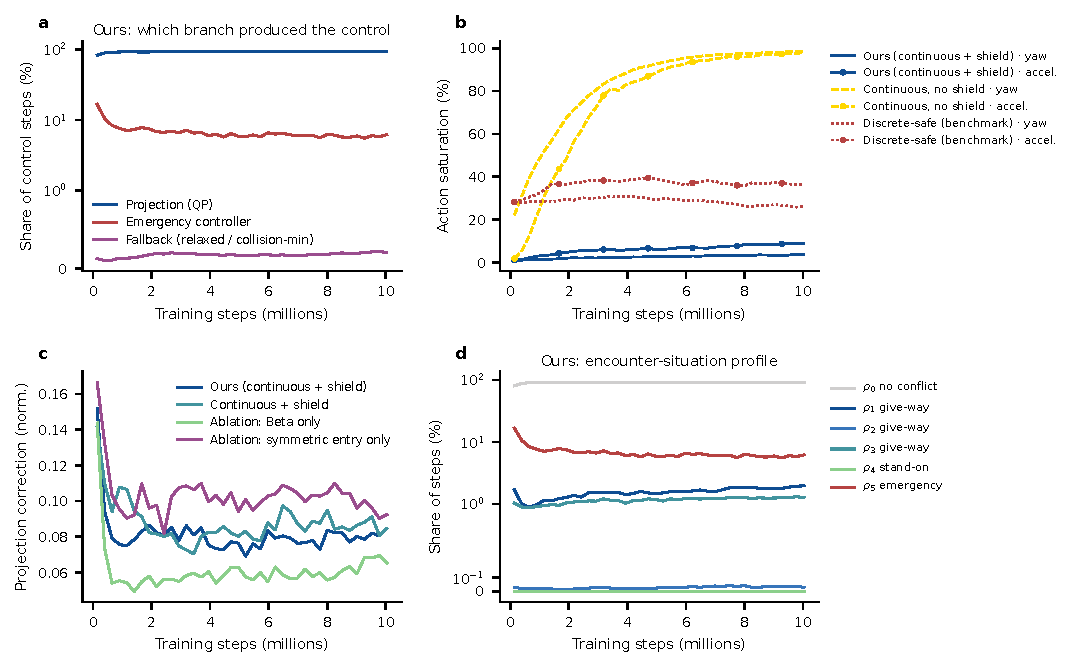
\includegraphics[width=\linewidth]{figs/fig5_shield_behaviour.pdf}
 \caption{Behavior of the shield. \capnote{In panel (d) the angle is the sector in which
 the convention defines each situation, \textbf{not} the measured bearing distribution of
 target vessels, and the radius is logarithmic. This figure is collected during training
 rather than at evaluation.}}
 \label{fig:shield}
\end{figure}

\subsection{Comparison with External Baselines}
\label{sec:res-ext}

Three geometric collision-avoidance controllers that need no training are run through the
same evaluation pipeline, on the same test set, at the same sample size
(Table~\ref{tab:ext}). The question here is not whether a learning method is stronger. It
is which dimensions a geometric method already covers.

The answer narrows the defensible claim to one dimension. The collision rate does not separate the two families, since the barrier function shield
also reaches $0.00\%$ here. The arrival rate and the smoothness columns are governed by
the terminal constraint and by the control range, and neither supports a reading in
favor of Ours. The real difference is in COLREGs violations, and almost all of it
comes from stand-on violations. These controllers aim only at avoiding contact, so they keep
maneuvering during periods in which the rules require course and speed to be held.
Violations are decided by the offline scorer from the bare situation predicates, so the
comparison is made under one condition. The claim of this paper against geometric methods
rests on this dimension alone. Ours records $0.53$ violations per episode against $4.95$
for the control barrier function filter at its best setting, which is a factor of $9.3$.
Almost all of that gap is in stand-on violations, at $0.36$ against $4.48$.

%------------------------------------------------------------------------------
\begin{table}[htbp]
 \caption{External geometric baselines. \capnote{Official test set, $N=600$.}}
 \label{tab:ext}
 \centering\small
 % 表体由 9 pt 提到 10 pt（TRB 硬要求 ≥10 pt）之后这张 9 列表会超宽 6.6 pt ⟹ 列间距收到 2 pt
 \setlength{\tabcolsep}{2pt}
 \begin{tabular*}{\linewidth}{@{\extracolsep{\fill}}llccccccc@{}}
  \toprule
  \multirow{2}{*}{Method} & \multirow{2}{*}{Control range} & \multirow{2}{*}{Arrival \%} & \multirow{2}{*}{Coll. \%}
   & \multicolumn{3}{c}{COLREGs violations / episode} & \multirow{2}{*}{Turn $\Delta$} & \multirow{2}{*}{Jerk} \\
  \cmidrule(lr){5-7}
   & & & & Total & Give-way & Stand-on & & \\
  \midrule
  \multirow{3}{*}{Control barrier function}
   & Policy range        & 70.17 & 0.00 & 4.95 & 0.47 & 4.48 & 0.00242 & 0.171 \\
   & Policy range, margin& 69.83 & 0.00 & 4.49 & 0.45 & 4.04 & 0.00235 & 0.167 \\
   & Actuator limits     & 69.33 & 0.00 & 6.48 & 0.52 & 5.97 & 0.00058 & 0.050 \\
  \addlinespace
  \multirow{2}{*}{PD controller}
   & Policy range    & 58.83 & 18.00 & 9.79 & 0.44 & 9.35 & 0.00492 & 0.310 \\
   & Actuator limits & 57.67 & 16.67 & 8.10 & 0.63 & 7.47 & 0.00032 & 0.040 \\
  \addlinespace
  \multirow{2}{*}{Velocity obstacle}
   & Policy range, margin & 57.00 & 0.00 & 8.20 & 0.50 & 7.70 & 0.00425 & 0.279 \\
   & Actuator limits      & 42.67 & 0.00 & 8.06 & 0.68 & 7.38 & 0.00128 & 0.071 \\
  \addlinespace
  Ours                     & Policy range & \multicolumn{7}{c}{(see Table~\ref{tab:main})} \\
  \bottomrule
 \end{tabular*}

 \vspace{4pt}
 \begin{minipage}{\linewidth}\small
 \textbf{Notes.} These controllers need no training and have no seed. Each is reported at its
 own best setting, tuned on a set that is disjoint from the one used here. The policy range
 is $\pm0.048$ and $\pm0.018$, the same authority as the trained policies, and the
 actuator limits are $\pm0.24$ and $\pm0.03$. Both are reported so that a difference in
 authority is not a confounder. \textbf{The arrival rate is not a measure of collision
 avoidance.} These controllers have no terminal alignment stage. They reach the goal
 position in $96.8\%$ to $99.7\%$ of episodes and then fail the terminal heading gate.
 \end{minipage}
\end{table}
%------------------------------------------------------------------------------


%==============================================================================
% §6 讨论 —— 对应中文稿 906–943 行
%==============================================================================
%------------------------------------------------------------------------------
\begin{figure}[htbp]
 \centering
 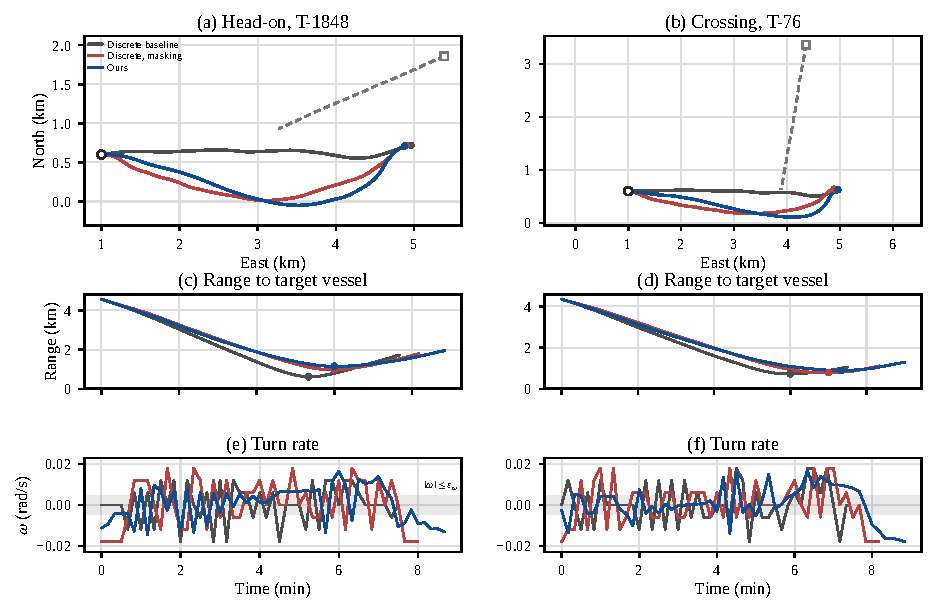
\includegraphics[width=\linewidth]{figs/fig6_trajectories.pdf}
 \caption{Tracks of three configurations in two encounters. \capnote{Scenarios are picked by
 geometry alone and never by outcome. Within each encounter type of the test set, the
 scenario shown is the one whose closest approach is smallest when both vessels hold their
 initial velocity, which is $7$~m for T-$1848$ and $2$~m for T-$76$. The seed is $s_0$, one of
 the three declared in advance, and the checkpoint is the last one of the run rather than the
 one selected on the validation set. The open circle is the start of the own vessel, the
 square is the start of the target vessel, and the dashed line is the recorded track of the
 target vessel. In (c) the dot marks the closest approach reached by each configuration and
 the dashed line is the closest approach under constant velocity. \textbf{This figure is a
 qualitative illustration and carries no quantitative claim.}}}
 \label{fig:traj}
\end{figure}
%------------------------------------------------------------------------------

\section{Discussion}
\label{sec:discussion}

\subsection{Two Points about the Mechanism} \noindent\textbf{Both refinements belong to
the continuous action space.}\ A quantized action space has no samples pushed past the
action box, and it has no channel whose differential entropy is unbounded above. Both
problems appear only after a COLREGs shield is moved into a continuous action space. The
ablation is therefore not the tuning of two hyperparameters. It repairs two defects
created by that move. \noindent\textbf{Recursive feasibility is not claimed.}\ A
reactive barrier function shield has no recursive feasibility proof under a $10$~s
zero-order hold. The clearable set of this work suggests one route to that property. The closed-loop
integration is not finished, so it is stated as a design direction and not as a
guarantee.

\subsection{What Projection Buys and What It Costs}
\label{sec:disc-grid}

Both sides of the exchange were measured directly, in exact arithmetic for the
resolution and on one machine for the cost.

The gain is in the resolution of a compliant turn. The rules require the heading change over
the maneuver window to reach a threshold, which converts to a smallest admissible
turn rate $\omega_{\mathrm{turn}}$. A continuous command reaches that value exactly.
A finite grid can only take the nearest grid point at or beyond it, so it always overshoots.
On the $7\times7$ grid reproduced here, the smallest available compliant turn rate is
$37.5\%$ above that value.

\noindent\textbf{That gap does not shrink monotonically as the grid is refined.}\ The
overshoot is set by the divisibility of $\omega_{\mathrm{turn}}$ by the grid spacing, not by
the spacing itself. A $5\times5$ grid overshoots by $3.1\%$ while a $7\times7$ grid overshoots by $37.5\%$. The common statement that a finer grid approaches
continuous control therefore does not hold for this task. Only a continuous command with
projection reaches the smallest admissible turn rate.

The cost is in computation, and it runs against intuition.
Enumerating and masking $K\times K$ commands costs time that grows with $K^2$. Even at $K=121$, which is $14{,}641$ commands, it stays well below the time
of one projection. \textbf{Projection is not the cheaper option.} Its justification is capability
rather than speed. Enumeration has no meaning on a continuous set, while projection is
feasible and lands exactly on the boundary of the constraint. The deployment cost of one
step is reported separately in Section~\ref{sec:res-shield}.

The difference in throttle resolution, where the discrete configurations have only seven
levels, is structural in the same way. It cannot be read directly from the throttle
increment column, because that column is also affected by the action-increment penalty, and
that penalty is active only in the continuous configurations. The attributable comparison
holds only among configurations that run the same penalty.


\subsection{What This Means for Putting Autonomous Vessels into Service}

Making compliance a projectable hard constraint changes more than the behavior of the
policy. It changes how this layer can be reviewed. When compliance is induced by training,
verification can only be statistical. A sample of scenarios is run, a violation frequency is
reported, and the conclusion moves with every version of the policy. When compliance holds
by construction, the object of verification becomes the constraint itself. A reviewer checks
whether the state machine classifies the situation correctly, whether the half-plane points
the way the clause requires, and whether the projection lands inside the feasible set. All
three can be checked step by step, and none of them depends on the training outcome. For
type approval and for accident review this is the more workable form. The reviewer does not
need to reproduce the training run.

The mechanism also does not require the existing control system to be replaced. It accepts a
desired control command from any source and returns the nearest compliant command. It can
therefore sit as a separate compliance layer above an existing autopilot or path-following
controller. Its online cost is one quadratic program per step, with two variables and at most
six constraints, and it needs no dedicated hardware. Deployment on current shipboard
computing platforms is realistic.

%==============================================================================
% §7 结论 —— 对应中文稿 945–952 行
%==============================================================================
\section{Conclusions}
\label{sec:conclusions}

The give-way clauses of COLREGs require a vessel to turn to a stated side, so compliance
cannot be verified from whether contact occurred. Existing work either buys a provable form
of compliance with a discrete action space and masking, or buys control resolution with
continuous commands and a soft reward. This paper shows that the exchange is not necessary.
The give-way clause is exactly a half-plane in the control plane. The premise that the
safe set must be enumerated can therefore be replaced by the premise that it is convex. A
projection-based safety shield is therefore brought to maritime COLREGs under continuous
control. Directional compliance on every give-way step where the projection is feasible holds
by construction, independently of the training outcome and of the seed. Any behavioral rule
that can be written as a convex constraint in the action space can follow the same route.

On the official test set of $600$ scenarios the median violation count of Ours is $0.53$
per episode. The discrete shielded baseline records $1.16$ and the strongest geometric
baseline records $4.95$. It is the only shielded configuration that meets the
convergence criterion on all eight seeds.

The boundaries of these conclusions are as follows. The shield does not guarantee freedom
from collision. Directional compliance holds on \textbf{every give-way step where the projection is
feasible}, not on every step. An emergency situation bypasses the constraint by design,
so the measured violation count is not zero. Propositions
\ref{prop:farfield} and \ref{prop:imminent} both assume that the target vessel holds its
velocity, and a maneuvering target vessel voids them. Neither the arrival rate nor smoothness
is claimed as a benefit, and smoothness cannot be attributed across action spaces because the
action-increment penalty is active only in the continuous configurations. Two biases in the reported numbers are known, namely checkpoint selection and
machine-to-machine variation. The main table is therefore reported in two versions, and
every configuration in one table is evaluated on one machine in one pass. On rule coverage, the directional requirements of Rules 13 to 17
and the stand-on obligation to hold course and speed are implemented. The stand-on duty to
take avoiding action on its own is not. The overtaking branch is implemented but the scenario
library contains no overtaking case, so it is untested. The discrete baseline is a
reimplementation, and its seed fragility is attributed to that reimplementation.

Three lines of work follow. The terminal constraint of the backup maneuver should be
wired into the deployed shield and verified in closed loop. Directional compliance
should be extended to several target vessels with a conflict resolution rule. The
far-field test should be implemented as an $O(1)$ early exit.

%==============================================================================
% 收尾四节 —— TRB 要求，对应中文稿 954–979 行
%==============================================================================
\section*{Acknowledgements}

The authors thank the CommonOcean benchmark and \citl{krasowski2024}{Krasowski and
Althoff 2024} for the public scenario library and the formalization of the rules. Both
made a comparison under one condition possible.

\section*{Author Contributions}

The authors confirm contribution to the paper as follows. Study conception and design: all
authors. Method and software: the first author. Data collection and analysis: the first and
second authors. Interpretation of results: all authors. Draft preparation: the first author.
All authors reviewed the results and approved the final version of the manuscript.

\section*{Conflict of Interest}

The authors declare that they have no known competing financial interests or personal
relationships that could have appeared to influence the work reported in this paper.

\section*{Funding}

The authors received no specific funding for this work.

%==============================================================================
\FloatBarrier   % 🔴 参考文献之前把所有待排浮动体清空，否则图表会插进文献表中间
\section*{References}

% [最后一轮补齐。量级约 40 条。**体例 = 官方规范的作者-年份制（Chicago author-date）**：
% 正文用 (Author, Year)，References 按第一作者姓氏字母序、悬挂缩进、不编号、不用上标。
% 锚点：对标工作（动力学 / 状态机 / 指标口径）· 安全盾在环强化学习与 zonotope 投影 · COLREGs 软奖励 ·
% 深度强化学习报告规范（种子敏感性 / 稳健指标）· CommonOcean 场景库 · COLREGs 公约原文 ·
% 控制障碍函数与预测式安全滤波 · 速度障碍。]

\refitem{\hypertarget{ref:altman1999}{}Altman, Eitan. 1999. \textit{Constrained Markov Decision Processes}. Boca Raton: Chapman \& Hall/CRC.}

\refitem{\hypertarget{ref:alshiekh2018}{}Alshiekh, Mohammed, Roderick Bloem, Rüdiger Ehlers, Bettina Könighofer, Scott Niekum, and Ufuk Topcu. 2018. ``Safe Reinforcement Learning via Shielding.'' In \textit{Proceedings of the AAAI Conference on Artificial Intelligence}.}

\refitem{\hypertarget{ref:ames2019}{}Ames, Aaron D., Samuel Coogan, Magnus Egerstedt, Gennaro Notomista, Koushil Sreenath, and Paulo Tabuada. 2019. ``Control Barrier Functions: Theory and Applications.'' In \textit{European Control Conference (ECC)}, 3420--3431.}

\refitem{\hypertarget{ref:benjamin2006}{}Benjamin, Michael R., John J. Leonard, Joseph A. Curcio, and Paul M. Newman. 2006. ``A Method for Protocol-Based Collision Avoidance Between Autonomous Marine Surface Craft.'' \textit{Journal of Field Robotics} 23 (5): 333--346.}

\refitem{\hypertarget{ref:cheng2018}{}Cheng, Yin, and Weidong Zhang. 2018. ``Concise Deep Reinforcement Learning Obstacle Avoidance for Underactuated Unmanned Marine Vessels.'' \textit{Neurocomputing} 272: 63--73.}

\refitem{\hypertarget{ref:chou2017}{}Chou, Po-Wei, Daniel Maturana, and Sebastian Scherer. 2017. ``Improving Stochastic Policy Gradients in Continuous Control with Deep Reinforcement Learning Using the Beta Distribution.'' In \textit{Proceedings of the International Conference on Machine Learning (ICML)}.}

\refitem{\hypertarget{ref:chun2021}{}Chun, D.-H., M.-I. Roh, H.-W. Lee, J. Ha, and D. Yu. 2021. ``Deep Reinforcement Learning-Based Collision Avoidance for an Autonomous Ship.'' \textit{Ocean Engineering} 234: 109216.}

\refitem{\hypertarget{ref:dalal2018}{}Dalal, Gal, Krishnamurthy Dvijotham, Matej Vecerik, Todd Hester, Cosmin Paduraru, and Yuval Tassa. 2018. ``Safe Exploration in Continuous Action Spaces.'' arXiv:1801.08757.}

\refitem{\hypertarget{ref:de2024}{}De Lellis, Francesco, Marco Coraggio, Giovanni Russo, Mirco Musolesi, and Mario di Bernardo. 2024. ``Guaranteeing Control Requirements via Reward Shaping in Reinforcement Learning.'' \textit{IEEE Transactions on Control Systems Technology}.}

\refitem{\hypertarget{ref:eriksen2019}{}Eriksen, Bjørn-Olav H., Morten Breivik, Erik F. Wilthil, Andreas L. Flåten, and Edmund F. Brekke. 2019. ``The Branching-Course Model Predictive Control Algorithm for Maritime Collision Avoidance.'' \textit{Journal of Field Robotics} 36.}

\refitem{\hypertarget{ref:fossen2011}{}Fossen, Thor I. 2011. \textit{Handbook of Marine Craft Hydrodynamics and Motion Control}. Chichester: John Wiley \& Sons.}

\refitem{\hypertarget{ref:garca2015}{}García, Javier, and Fernando Fernández. 2015. ``A Comprehensive Survey on Safe Reinforcement Learning.'' \textit{Journal of Machine Learning Research} 16: 1437--1480.}

\refitem{\hypertarget{ref:grover2023}{}Grover, Jaskaran, Changliu Liu, and Katia Sycara. 2023. ``The Before, During, and After of Multi-Robot Deadlock.'' \textit{International Journal of Robotics Research}.}

\refitem{\hypertarget{ref:heiberg2022}{}Heiberg, Amalie, Thomas Nakken Larsen, Eivind Meyer, Adil Rasheed, Omer San, and Damiano Varagnolo. 2022. ``Risk-Based Implementation of COLREGs for Autonomous Surface Vehicles Using Deep Reinforcement Learning.'' \textit{Neural Networks} 152: 17--33. arXiv:2112.00115.}

\refitem{\hypertarget{ref:huang2019}{}Huang, Yamin, Linying Chen, and P. H. A. J. van Gelder. 2019. ``Generalized Velocity Obstacle Algorithm for Preventing Ship Collisions at Sea.'' \textit{Ocean Engineering} 173: 142--156.}

\refitem{\hypertarget{ref:imo1972}{}IMO (International Maritime Organization). 1972. \textit{Convention on the International Regulations for Preventing Collisions at Sea (COLREGs)}. London: IMO.}

\refitem{\hypertarget{ref:johansen2016}{}Johansen, Tor A., Tristan Perez, and Andrea Cristofaro. 2016. ``Ship Collision Avoidance and COLREGS Compliance Using Simulation-Based Control Behavior Selection with Predictive Hazard Assessment.'' \textit{IEEE Transactions on Intelligent Transportation Systems} 17 (12): 3407--3422.}

\refitem{\hypertarget{ref:kim2024}{}Kim, Kyungmin, Davide Corsi, Andoni Rodríguez, JB Lanier, Benjamí Parellada, Pierre Baldi, César Sánchez, and Roy Fox. 2024. ``Realizable Continuous-Space Shields for Safe Reinforcement Learning.'' arXiv:2410.02038.}

\refitem{\hypertarget{ref:kochdumper2023}{}Kochdumper, Niklas, Hanna Krasowski, Xiao Wang, Stanley Bak, and Matthias Althoff. 2023. ``Provably Safe Reinforcement Learning via Action Projection Using Reachability Analysis and Polynomial Zonotopes.'' \textit{IEEE Open Journal of Control Systems} 2.}

\refitem{\hypertarget{ref:krasowski2022}{}Krasowski, Hanna, and Matthias Althoff. 2022. ``CommonOcean: Composable Benchmarks for Motion Planning on Oceans.'' In \textit{Proceedings of the IEEE International Conference on Intelligent Transportation Systems (ITSC)}, 1676--1682. DOI: 10.1109/ITSC55140.2022.9921925. \url{https://commonocean.cps.cit.tum.de/}.}

\refitem{\hypertarget{ref:krasowski2024}{}Krasowski, Hanna, and Matthias Althoff. 2024. ``Provable Traffic Rule Compliance in Safe Reinforcement Learning on the Open Sea.'' \textit{IEEE Transactions on Intelligent Vehicles} 9 (12): 7617--7634. arXiv:2402.08502.}

\refitem{\hypertarget{ref:kufoalor2020}{}Kufoalor, D. K. M., Tor A. Johansen, Edmund F. Brekke, A. Hepsø, and K. Trnka. 2020. ``Autonomous Maritime Collision Avoidance: Field Verification of Autonomous Surface Vehicle Behavior in Challenging Scenarios.'' \textit{Journal of Field Robotics} 37.}

\refitem{\hypertarget{ref:kuwata2014}{}Kuwata, Yoshiaki, Michael T. Wolf, Dimitri Zarzhitsky, and Terrance L. Huntsberger. 2014. ``Safe Maritime Autonomous Navigation with COLREGS, Using Velocity Obstacles.'' \textit{IEEE Journal of Oceanic Engineering} 39 (1): 110--119.}

\refitem{\hypertarget{ref:lee2025}{}Lee, Changyu, Jinwook Park, and Jinwhan Kim. 2026. ``Efficient COLREGs-Compliant Collision Avoidance Using Turning Circle-Based Control Barrier Function.'' \textit{Mechatronics} 117.}

\refitem{\hypertarget{ref:markgraf2026}{}Markgraf, Hannah, Shambhuraj Sawant, Hanna Krasowski, Lukas Schäfer, Sébastien Gros, and Matthias Althoff. 2026. ``Safe Reinforcement Learning Using Action Projection: Safeguard the Policy or the Environment?'' \textit{Transactions on Machine Learning Research}.}

\refitem{\hypertarget{ref:meyer2020}{}Meyer, Eivind, Amalie Heiberg, Adil Rasheed, and Omer San. 2020. ``COLREG-Compliant Collision Avoidance for Unmanned Surface Vehicle Using Deep Reinforcement Learning.'' \textit{IEEE Access} 8.}

\refitem{\hypertarget{ref:mller2025}{}Müller, Henrik, and Daniel Kudenko. 2025. ``Improving the Effectiveness of Potential-Based Reward Shaping in Reinforcement Learning.'' In \textit{Proceedings of the International Conference on Autonomous Agents and Multiagent Systems (AAMAS)}. arXiv:2502.01307.}

\refitem{\hypertarget{ref:mller2026}{}Müller, Marlon, Florian Finkeldei, Hanna Krasowski, Murat Arcak, and Matthias Althoff. 2026. ``Falsification-Driven Reinforcement Learning for Maritime Motion Planning.'' \textit{Ocean Engineering} 361: 125579.}

\refitem{\hypertarget{ref:ng1999}{}Ng, Andrew Y., Daishi Harada, and Stuart Russell. 1999. ``Policy Invariance Under Reward Transformations: Theory and Application to Reward Shaping.'' In \textit{Proceedings of the International Conference on Machine Learning (ICML)}, 278--287.}

\refitem{\hypertarget{ref:oh2025}{}Oh, Donggeon David, Duy P. Nguyen, Haimin Hu, and Jaime F. Fisac. 2025. ``Provably Optimal Reinforcement Learning under Safety Filtering.'' arXiv:2510.18082.}

\refitem{\hypertarget{ref:patil2026}{}Patil, Mayur S., Nataraj Sudharsan, Veneela Ammula, Jude Tomdio, Jin Wang, Michael Kei, Sivakumar Rathinam, and Prabhakar R. Pagilla. 2026. ``COLREGs Compliant Collision Avoidance and Grounding Prevention for Autonomous Marine Navigation.'' arXiv:2603.02484.}

\refitem{\hypertarget{ref:pizarro2025}{}Pizarro Bejarano, Federico, Lukas Brunke, and Angela P. Schoellig. 2025. ``Safety Filtering While Training: Improving the Performance and Sample Efficiency of Reinforcement Learning Agents.'' \textit{IEEE Robotics and Automation Letters}.}

\refitem{\hypertarget{ref:raffin2021}{}Raffin, Antonin, Ashley Hill, Adam Gleave, Anssi Kanervisto, Maximilian Ernestus, and Noah Dormann. 2021. ``Stable-Baselines3: Reliable Reinforcement Learning Implementations.'' \textit{Journal of Machine Learning Research} 22 (268): 1--8.}

\refitem{\hypertarget{ref:sarhadi2022}{}Sarhadi, Pouria, Wasif Naeem, and Nikolaos Athanasopoulos. 2022. ``A Survey of Recent Machine Learning Solutions for Ship Collision Avoidance and Mission Planning.'' \textit{IFAC-PapersOnLine}.}

\refitem{\hypertarget{ref:schulman2016}{}Schulman, John, Philipp Moritz, Sergey Levine, Michael I. Jordan, and Pieter Abbeel. 2016. ``High-Dimensional Continuous Control Using Generalized Advantage Estimation.'' In \textit{International Conference on Learning Representations (ICLR)}.}

\refitem{\hypertarget{ref:schulman2017}{}Schulman, John, Filip Wolski, Prafulla Dhariwal, Alec Radford, and Oleg Klimov. 2017. ``Proximal Policy Optimization Algorithms.'' arXiv:1707.06347.}

\refitem{\hypertarget{ref:shen2019}{}Shen, Haiqing, Hirotada Hashimoto, Akihiko Matsuda, Yuuki Taniguchi, Daisuke Terada, and Chen Guo. 2019. ``Automatic Collision Avoidance of Multiple Ships Based on Deep Q-Learning.'' \textit{Applied Ocean Research} 86: 268--288.}

\refitem{\hypertarget{ref:trott2019}{}Trott, Alexander, Stephan Zheng, Caiming Xiong, and Richard Socher. 2019. ``Keeping Your Distance: Solving Sparse Reward Tasks Using Self-Balancing Shaped Rewards.'' In \textit{Advances in Neural Information Processing Systems (NeurIPS)}.}

\refitem{\hypertarget{ref:vaaler2024}{}Vaaler, Aksel, Svein Jostein Husa, Daniel Menges, Thomas Nakken Larsen, and Adil Rasheed. 2024. ``Modular Control Architecture for Safe Marine Navigation: Reinforcement Learning and Predictive Safety Filters.'' arXiv:2312.01855.}

\refitem{\hypertarget{ref:wabersich2021}{}Wabersich, Kim P., and Melanie N. Zeilinger. 2021. ``A Predictive Safety Filter for Learning-Based Control of Constrained Nonlinear Dynamical Systems.'' \textit{Automatica} 129: 109597.}

\refitem{\hypertarget{ref:zhao2019}{}Zhao, Luman, and Myung-Il Roh. 2019. ``COLREGs-Compliant Multiship Collision Avoidance Based on Deep Reinforcement Learning.'' \textit{Ocean Engineering} 191: 106436.}


\end{document}
